\documentclass[11pt, oneside, a4paper, titlepage, french]{article}
\usepackage[T1]{fontenc}     % Support des césures comportant des accents
\usepackage{calc}            % Manipulation facile des tailles
\usepackage{graphicx}        % Figures basiques
\usepackage{lmodern}         % Meilleure police
\usepackage[utf8]{inputenc}  % Support de l'encodage utf-8
\usepackage{fancyvrb}
\usepackage{hyperref}
\usepackage{url}
\usepackage{xcolor}
\usepackage{svg}
\usepackage{float}
\usepackage[french]{babel}
\usepackage{listings}
\usepackage{array}
\selectlanguage{french}

\newcommand{\imagepath}{logos/}
\newcommand{\createimagepath}[1]{\imagepath#1}

\topmargin      -10mm
\textheight     224mm
\footskip       20mm
\hoffset        -10mm
\textwidth      146mm
\hypersetup{
    colorlinks = true,
    linkcolor = blue,
    urlcolor = cyan
}

\lstset{
  basicstyle=\ttfamily,
  columns=fullflexible,
  showstringspaces=false,
  commentstyle=\color{gray}\upshape
}

\lstset{%
    inputencoding=utf8,
    extendedchars=true,
    literate=%
    {é}{{\'e}}{1}%
    {è}{{\`e}}{1}%
    {à}{{\`a}}{1}%
    {ç}{{\c{c}}}{1}%
    {œ}{{\oe}}{1}%
    {ù}{{\`u}}{1}%
    {É}{{\'E}}{1}%
    {È}{{\`E}}{1}%
    {À}{{\`A}}{1}%
    {Ç}{{\c{C}}}{1}%
    {Œ}{{\OE}}{1}%
    {Ê}{{\^E}}{1}%
    {ê}{{\^e}}{1}%
    {î}{{\^i}}{1}%
    {ô}{{\^o}}{1}%
    {û}{{\^u}}{1}%
    {ë}{{\¨{e}}}{1}%
    {û}{{\^{u}}}{1}%
    {â}{{\^{a}}}{1}%
    {Â}{{\^{A}}}{1}%
    {Î}{{\^{I}}}1
}

\begin{document}
%----------------------------------------------------------------------------------%

%--- page de garde ---%
\begin{titlepage}
% garde.tex
% 
% Auteur: Mohamed Habib Essoussi <mohamedhabib.essoussi@gmail.com>
%
% Date de création: 22/05/2012
%
%
% Ce fichier est développé afin de faciliter la mise en oeuvre de la page de garde
% des rapports de stage en latex pour les étudiants de TELECOM SudParis et qui est
% conforme au design décrit aux annexes du guide des stages pour les étudiants en
% 3eme année. 
%
%
% Il suffit de remplacer les valeurs ci-dessous par les votres:
\newcommand{\nomprenom}{% Votre nom et prénom
    \fontsize{14}{14}\selectfont Rémy ZIRNHELD
}
\newcommand{\nomEntreprise}{% Nom de l'entreprise en majuscule
    \fontsize{16}{16}\selectfont Institut National de la Statistique et des Études Économiques
}

\newcommand{\nomAdresseEntreprise}{% nom, adresse de l'entreprise 
    \fontsize{12}{12}\selectfont Institut National de la Statistique et des Études Économiques, 88 Avenue Verdier, 92120 Montrouge.
}

\newcommand{\titreMission}{% Le titre de la mission
    \fontsize{14}{14}\selectfont Élaboration d'un service de reconnaissance d'entités nommées dans les publications de l'Insee
}

\newcommand{\nomDirecteurStage}{% Le nom et le prénom du directeur de stage auprès de l'entreprise
    \fontsize{12}{12}\selectfont Franck COTTON
}

\newcommand{\nomConseillerStage}{% Le nom et le prénom du conseiller de stage à TSP
    \fontsize{12}{12}\selectfont Amel BOUZEGHOUB
}

\newcommand{\anneeUniversitaire}{% L'année universitaire en format 20xx/20xx
    \fontsize{15}{15}\selectfont 2018/2019
}

\newcommand{\dateDebut}{% Date du début
    \fontsize{12}{12}\selectfont 04/03/2019
}

\newcommand{\dateFin}{% Date de la fin
    \fontsize{12}{12}\selectfont 30/08/2019
}

% Il faudra créer les deux commandes suivantes le plus tôt que possible dans votre
% projet latex.

%\newcommand{\imagepath}{% Saisissez ici le répertoire de vos logos
%logos/
%}
%\newcommand{\createimagepath}[1]{\imagepath#1} % A ne pas modifier

%%%% FIN DES COMMANDES DE CONFIGURATION %%%%
% !!! N'EDITEZ PAS CE QUI SUIT - SAUF EN CAS DE BESOIN !!!
% ============================================================================ %

\newpage 
\thispagestyle{empty}

%%%%%%%%%%%%%%%%%%%%%%%%%%%%%%%%%%%%%%%%%%%%%%%%%%%%%%%%%%%%%%%%%%%%%%%%%%%%%%%%
%				PREMIER GROUPE				       %
%%%%%%%%%%%%%%%%%%%%%%%%%%%%%%%%%%%%%%%%%%%%%%%%%%%%%%%%%%%%%%%%%%%%%%%%%%%%%%%%

% ============================================================================ %
%	LOGO_TELECOM_SUDPARIS				    ANNEE 20XX/20XX    %
% ============================================================================ %	
	\begingroup
		\begin{tabular}{ll}
		% LOGO DE TELECOM SUDPARIS
  			\begin{minipage}[c]{0.0\textwidth}
				\begin{flushleft}
				\includegraphics[width=3cm]{%
					\createimagepath{Logo_Telecom_sudparis.jpg}}
				\end{flushleft}
			\end{minipage}
 		 & 
		% ANNEE UNIVERSITAIRE
		\begin{minipage}[c]{1.0\textwidth}
               		 \begin{flushright}
			   	\textbf{ ANNEE \anneeUniversitaire}	
                	 \end{flushright}
       		 \end{minipage}
	          \hspace{\stretch{1}}
		\end{tabular}
       		 \vskip 4.0em
	\endgroup


%%%%%%%%%%%%%%%%%%%%%%%%%%%%%%%%%%%%%%%%%%%%%%%%%%%%%%%%%%%%%%%%%%%%%%%%%%%%%%%%
%		         	DEUXIEME GROUPE				       %
%%%%%%%%%%%%%%%%%%%%%%%%%%%%%%%%%%%%%%%%%%%%%%%%%%%%%%%%%%%%%%%%%%%%%%%%%%%%%%%%

% ============================================================================ %
%		RAPPORT de "MISSION  en ENTREPRISE"			       %
%									       %
%		  	   présenté par					       %
%			   \nomprenom					       %
%									       %
%		Mission effectuée du \dateDebut au \dateFin chez	       %
%			    \nomEntreprise				       %
%									       %
%			    sujet de la mission:			       %
%									       %
%		________________________________________		       %
%		| 		\titreMission		|		       %
%		_________________________________________		       %
%									       %
% ============================================================================ %

	\begingroup
		\begin{center}
			\textbf{\Large{RAPPORT de "MISSION en ENTREPRISE"}}	
        		\vskip 2.0em

			présenté par:					  	
        		\vskip 2.0em
			\textbf{\nomprenom}					  	
			
        		\vskip 3.0em
			{Mission effectuée de \dateDebut au \dateFin à l'}  	
        		\vskip 2.0em
			\textbf{\nomEntreprise}	
        		\vskip 3.5em

			Sujet de la mission:				 	
		\end{center}

		 % CADRE POUR LE TITRE DE LA MISSION
		 \parbox[b]{\textwidth}{%
          	  \hrule height 1.5pt
            	   \vrule width 1.5pt
                	\hspace{1.80cm}
            		\parbox[b]{\textwidth-4cm}{%
            		\vspace{0.6em}
            		\center\large{%
               			\textbf{\titreMission}
              	 	 }\endcenter
           		 \vspace{0.6em}}
           		 \hspace{1.80cm}
           		 {\vrule width 1.5pt}
            	    \hrule height 1.5pt
                    }
        	\vskip 3.4em
	\endgroup

%%%%%%%%%%%%%%%%%%%%%%%%%%%%%%%%%%%%%%%%%%%%%%%%%%%%%%%%%%%%%%%%%%%%%%%%%%%%%%%%
%		         	TROISIEME GROUPE			       %
%%%%%%%%%%%%%%%%%%%%%%%%%%%%%%%%%%%%%%%%%%%%%%%%%%%%%%%%%%%%%%%%%%%%%%%%%%%%%%%%

% ============================================================================ %
% Directeur de stage: \nomDirecteurStage				       %
% Conseiller de Stage: \nomConseillerStage				       %
% ============================================================================ %

\begingroup
	Directeur de stage: \textbf{\nomDirecteurStage}						       
        \vskip 1.0em
	Conseillère de Stage: \textbf{\nomConseillerStage}	
\endgroup

        \vskip 3.4em

%%%%%%%%%%%%%%%%%%%%%%%%%%%%%%%%%%%%%%%%%%%%%%%%%%%%%%%%%%%%%%%%%%%%%%%%%%%%%%%%
%		         	BAS DE PAGE				       %
%%%%%%%%%%%%%%%%%%%%%%%%%%%%%%%%%%%%%%%%%%%%%%%%%%%%%%%%%%%%%%%%%%%%%%%%%%%%%%%%

% ============================================================================ %
% ____________________________________________________________________________ %
% Travail effectué pour la société: \nomEntrepriseComplet		       %
% ============================================================================ %

\begingroup
        \hrule height 1.0pt
        \vskip 0.5em
	Travail effectué pour l' \nomAdresseEntreprise
\endgroup
\newpage

\end{titlepage}

%--- blanc ---%
\thispagestyle{empty}
\newpage
%----------------------------------------------------------------------------------%

%--- résumé & abstract ---%
\section*{Résumé}
Est-il possible de reconnaître automatiquement des concepts abstraits dans des publications ? C'est en tout cas le défi qui m'a été lancé par l'Insee pour mon stage de fin d'études.
\newline

Une branche du traitement du langage naturel consiste à reconnaître automatiquement des entités dans du texte de manière par exemple à identifier des personnes, des régions géographiques ou encore des monnaies. Ce rapport décrit les différentes étapes du déroulé du stage, de l'étude du domaine de la reconnaissance d'entités nommées jusqu'à la mise en place d'un Web Service. Il expose également toutes les compétences, tant techniques que transversales, mises en oeuvre dans l'élaboration d'un service de reconnaissance d'entités nommées.
\newpage

\section*{Abstract}
Is it possible to automatically recognize abstract concepts in editions? This is the challenge that INSEE presented to me for my end-of-study internship.
\newline

A field of natural language processing is to automatically recognize entities in a text in order to identify, for example, persons, geographical locations or currencies. This report describes the different stages of the internship, from the study of the field of named entity recognition to the implementation of a Web Service. It also outlines all the skills, both technical and transversal, required to develop a service for named entitiy recognition.
\newpage

%--- remerciements ---%
\section*{Remerciements}
Un grand merci d'abord à Franck Cotton pour m'avoir proposé ce stage et avoir suivi son avancement tout au long de ces six mois.
\newline

Je remercie également Juliette Fourcot qui m'a encadré et aidé à de nombreuses reprises, tant sur des aspects techniques qu'organisationnels.
\newline

Merci également à Amel Bouzeghoub pour avoir été ma conseillère tout au long de ce stage.
\newline

Je remercie de plus Mélinée Treppoz-Salomon, Frédéric Comte, Olivier Levitt et Éric Sigaud. Mélinée pour s'être rendue disponible pour m'aider dans la prise en main des outils mis à disposition. Frédéric et Olivier pour leurs savoir et leur pédagogie, qui m'ont permis de grandement améliorer la qualité des livrables logiciels. Éric pour sa bienveillance et son expertise.
\newline

Merci à Thomas Dubois et son équipe pour l'intérêt porté au projet.
\newline

Un grand merci à Yousra Cherkaoui Tangi pour la relecture de ce rapport.
\newline

Et enfin merci à vous qui lisez ce rapport.
\newpage

%--- table des matières ---%
\tableofcontents
\newpage

%----------------------------------------------------------------------------------%

%--- introduction ---%
\section*{Introduction}
Ce stage a été proposé par M. Franck Cotton, conseiller scientifique de la Direction du Système d'Information de l'Insee. Un des objectifs de l'Insee était de s'approprier les dernières évolutions en matière de traitement du langage naturel, en particulier dans le domaine de la reconnaissance d'entités nommées. Une entité nommée peut désigner une organisation, un lieu, une date ou encore une personne. La finalité est d'enrichir l'information contenue dans les publications par des éléments de contexte spécifique au domaine métier de l'Insee. Avec l'utilisation récente des réseaux de neurones dans le traitement du langage naturel, ce domaine a beaucoup évolué. Les traitements sont de plus en plus performants et proposent davantage de fonctionnalités. Ce projet est l'occasion de mettre en application ces nouvelles technologies du traitement du langage naturel, en construisant un premier service de reconnaissance d'entités nommées. Ce service devra être capable de reconnaître, dans les publications de l'Insee, des concepts généraux tels que des dates ou des lieux, mais aussi les concepts statistiques de l'Insee.
\newline

Après une définition du projet et de l'environnement de travail, nous décrirons les enjeux de l'utilisation du traitement du langage naturel à l'Insee. Nous présenterons ensuite le détail du développement d'un premier service, avant d'en faire le bilan.
\newpage

\section{L'Insee, environnement propice à la Data Science}
Ce stage a été proposé par l'Insee dans le cadre de l'une de ses missions, à savoir, celle de la diffusion de l'information statistique. Accueilli à la direction générale, j'ai eu l'occasion de découvrir le fonctionnement d'une grande administration française ainsi que son appropriation des techniques du \textit{Big Data} et des \textit{Data sciences}.

\subsection{Environnement professionnel}

\subsubsection{Présentation de l'Insee}
\vspace{10pt}
\begin{center}

\includegraphics[scale=0.12]{images/Logo_Insee.png} 
\end{center}

L'Institut national de la statistique et des études économiques (Insee), créé par la loi des finances du 27 avril 1946, est une administration publique rattachée au ministère de l'Économie et des Finances. Il est dirigé actuellement par Monsieur Tavernier.
\newline

L'Insee a pour mission de collecter, analyser et diffuser des informations sur l'économie et la société française sur l'ensemble de son territoire. Il organise les campagnes de recensement de la population, réalise la comptabilité nationale, mène des enquêtes sur les ménages ou les entreprises françaises, mesure les principaux indicateurs de l'économie comme le taux de chômage ou le taux de croissance. Il gère également un certain nombre de répertoires~:
\begin{enumerate}
    \item Le répertoire Sirene~: il permet d'identifier les entreprises.
    \item La base des répertoires des personnes physiques~: elle permet de certifier les états civils des individus, leur attribuer un numéro d'inscription au répertoire communément appelé «~numéro de sécurité sociale~».
    \item Le Répertoire électoral unique~: il a pour finalité la gestion du processus électoral et la fiabilisation des listes électorales.
\end{enumerate}

L'Insee est de plus en charge de nomenclatures officielles~: les Professions et Catégories Socioprofessionnelles (PCS) ainsi que le Code Officiel Géographique (COG).
\newline

L'Institut a aussi pour mission de diffuser l'information statistique à un public le plus large possible, notamment au travers de son site internet. Sont disponibles via ce portail les informations relatives à tous les services décrits précédemment. Ces informations permettent d'aider les entreprises, les particuliers, les chercheurs, les administrations et les pouvoirs publics en les éclairant sur la situation et les enjeux économiques, démographiques et sociaux à l'échelle locale comme à l'échelle nationale. Concernant la diffusion à l'international, l'Insee contribue activement aux travaux européens portés par Eurostat, en charge de la statistique européenne officielle.
\newline

Enfin, l’Insee coordonne et anime le réseau du Service Statistique Publique (SSP) composé de services statistiques dédiés au sein des ministères (justice, travail, environnement, etc.). Elle travaille également avec d’autres organes administratifs ayant des activités statistiques (Banque de France, Ined, etc.).
\newline

L'organisation administrative de l'Insee comprend~:
\begin{enumerate}
    \item Une Direction Générale (DG) située à Montrouge (92) qui assure des tâches de conception, de coordination et d'étude au niveau national. Le centre statistique de Metz et le centre de formation de Libourne sont des entités de la direction générale implantées en région.
    \item Treize Directions Régionales (DR) en métropole et deux dans les DOM.
\end{enumerate}

\subsubsection*{La Direction du Système d'Information}

La gouvernance des sujets informatiques de l’Insee est confiée à la Direction du Système d'Information (DSI). 
\newline

Les missions de la DSI sont d’assurer la construction, les évolutions, l'exploitation et la disponibilité du système d'information de l'Insee.
\newline

La direction comporte trois entités qui pilotent respectivement les problématiques~:
\begin{enumerate}
    \item d'exploitation du SI~: Département de la Production et de l'Infrastructure Informatique (DPII)
    \item de développement du SI~: Département du Développement du SI (DDSI)
    \item de stratégie et de cohérence du SI~: unité de l'innovation et de la stratégie du système d'information ( UnISSI), au sein de laquelle se trouve la Division innovation et instruction technique.
    \newline
\end{enumerate}

En outre plusieurs services sont déconcentrés au sein d’établissements régionaux~:
\begin{enumerate}
    \item  Le Centre d’Exploitation Informatique (CEI) intégré au centre statistique de Metz et le Service National des Supports Informatiques (SNSI) situé à Nantes, tous deux sous la responsabilité fonctionnelle du DPII.
    \item Quatre services nationaux de développement informatiques (SNDI) situés à Lille, Nantes, Orléans et Paris et un Pôle Gestion de Contenu et Outils Collaboratifs (PGCOC) situé à Aix-en-Provence, sous la responsabilité fonctionnelle du DDSI.
\end{enumerate}

\subsubsection{La Division Innovation et Instruction Technique}
Je suis accueilli dans la Division innovation et instruction technique (Diit), qui comprend quatre agents. Créée en 2018, elle fait partie de l'UnISSI. La mission de la Diit est d'offrir un cadre propice à l'innovation à l'Insee, et d'accompagner la transformation numérique de l'Institut autour de cinq grandes orientations~:
\begin{enumerate}
    \item La collaboration
    \item La statistique reproductible
    \item L'open source 
    \item La Data science
    \item Le développement d'applications orienté DataOps
    \newline
\end{enumerate}

Actuellement, la division Innovation et instruction technique assure la maîtrise d’ouvrage et la maîtrise d’œuvre de la plate-forme innovation, dont une description plus détaillée est donnée section \ref{section 2.2.1}. Le maintenance de cette infrastructure s’appuie également sur du volontariat de quelques agents dans différentes entités de l’Insee. En particulier, l’intégration de certains services relève d’agents externes à la Diit, y compris hors DSI. 
\newline

Bien que j'effectue mon travail au sein de l'équipe, comme mon sujet s'intègre dans leur thématique de l'Open Source et de la Data science, il est supervisé par Franck Cotton, conseiller scientifique auprès du DSI et à l'origine du projet. 
\newline

Le SSP Lab, unité qui travaille sur l'utilisation de la Data science pour les services de statistique publique, se montre également intéressé par mon projet. Par ailleurs les membres du SSP Lab travaillent régulièrement avec la Diit, à l'occasion de hackaton sur la Datascience par exemple. J'ai donc l'occasion de travailler avec des personnes aux profils variés~:
\vspace{10pt}
\begin{figure}[H]
  \centering
  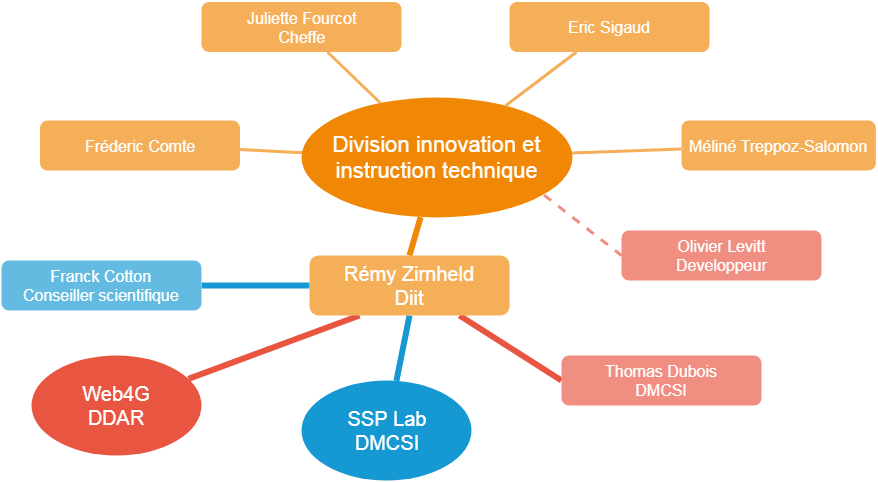
\includegraphics[scale=0.45]{images/Organigramme-stage.png}
  \caption{Liste des personnes m'aidant sur le projet}
  \label{fig:Organigramme}
\end{figure}

\vspace{20pt}

\begin{itemize}
    \item \textbf{Franck Cotton}~: Conseiller scientifique auprès de la Direction du Système d'Information. À l'origine du projet, il est le directeur du stage et me guide dans mes réflexions.
    \vspace{5pt}
    \item \textbf{Juliette Fourcot}~: Cheffe de la Diit, elle remplace Franck pour mon suivi lors de ses nombreux déplacements. Elle m'a apporté, tout au long du stage une aide précieuse, tant sur les aspects organisationnels que techniques.
    \vspace{5pt}
    \item \textbf{Eric Sigaud}~: Membre de la Diit, il m'apporte une aide technique sur l'utilisation de la plateforme innovation, ainsi que sur l'utilisation d'XSLT pour le traitement des fichiers XML. Il m'apporte également un oeil éclairé pour les diverses présentations que j'ai dû préparer durant ce stage.
    \vspace{5pt}
    \item \textbf{Frédéric Comte}~: Également membre de la division innovation et principal architecte de la plateforme, il m'apporte beaucoup de connaissances techniques sur la plateforme. J'ai notamment eu l'occasion de changer et configurer des nouveaux serveurs.
    \vspace{5pt}
    \item \textbf{Mélinée Treppoz-Salomon}~: Membre de l'équipe innovation, elle m'aide sur l'utilisation de la plateforme ainsi que sur mes diverses présentations.
    \vspace{5pt}
    \item \textbf{Olivier Levitt}~: Développeur au Recensement de la Population (RP). Son expertise dans le développement d'application contribue largement au bon déroulement du projet.
    \vspace{5pt}
    \item \textbf{Thomas Dubois}~: Chef de projet statistique à l'unité qualité, incluse dans la Direction de la Méthodologie et de la Coordination Statistique et Internationale (DMCSI). Chef de l'équipe en charge du Référentiel des Métadonnées Statistiques (voir \ref{section 1.2.1}), il fournit un regard métier sur le projet.
    \vspace{5pt}
    \item \textbf{L'équipe Web4g}~: En charge du site insee.fr, l'équipe Web4g me fournit des informations sur la structure des publications, ainsi qu'un accès à la base de données qui les référence. Elle dépend fonctionnellement de la Direction de la Diffusion et de l'Action Régionale (DDAR), qui gère notamment le site web de l'Insee.
    \vspace{5pt}
    \item \textbf{Le SSP Lab}~: Laboratoire du Service Statistique Public. Cette équipe travaille sur les nouvelles méthodes (Datasciences et Big Data), et suit les avancées de mon projet.
    \newline
\end{itemize}

Si ce projet est réalisé par moi-même sur le plan technique, je suis accompagné dans ma démarche par ces différents acteurs.
\label{section 1.1.2}

\subsection{Le cadre du projet}

\subsubsection{Le référentiel des métadonnées statistiques}
Parmi les entités nommées à reconnaître dans les publications figurent des concepts statistiques. Ces concepts sont référencés dans le Référentiel des Métadonnées Statistiques (RMéS) de l'Insee, disponible sur le site \href{http://rdf.insee.fr/sparql}{rdf.insee.fr} \cite{rdf.insee.fr} au format RDF. Les concepts y sont décrits à l'aide de plusieurs champs~: libellé, libellé alternatif, le plus souvent un acronyme, définitions et notes permettent de les identifier. Les concepts statistiques sur lesquels j'ai travaillé sont au nombre de 1162. Des liens sémantiques entre concepts enrichissent également la sémantique des concepts. En voici un exemple~:
\begin{figure}[H]
    \centering
    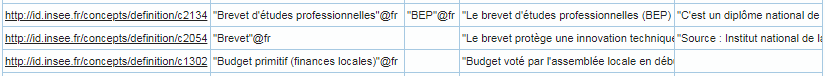
\includegraphics[scale=0.68]{images/Exemple-RMeS.png}
    \caption{Exemple de concepts de la base RMéS}
    \label{fig:exemple-rmés}
\end{figure}

Afin d'avoir une meilleure vision de ce que doit être une telle base, et à la demande de Franck, j'ai effectué une comparaison avec différentes bases de concepts au format rdf également~: 
\begin{itemize}
    \item Le thesaurus de l'\href{http://vocabularies.unesco.org/browser/thesaurus/en/?clang=fr}{Unesco} \cite{unesco}
    \item Le base de la \href{https://data.bnf.fr/current/sparql.html}{Bibliothèque nationale de France} \cite{bnf}
    \item La base de concepts d'\href{https://pro.europeana.eu/page/linked-open-data}{Europeana} \cite{europeana-rdf}
    \newline
\end{itemize}

Plusieurs particularités sont à noter~: tout d'abord, les concepts statistiques ont des libellés et définitions de tailles variées, contrairement aux autres bases où les définitions sont courtes et où la taille des libellés est homogène. Cette spécificité vient du fait que les contenus sont rédigés par les responsables métiers du domaine dans lequel ils sont mobilisés. Certaines informations contenues dans les libellés devraient être traduites sous la forme de triplet RDF~: «~Chômeur (BIT)~» et «~Chômeur (recensement de la population)~» sont deux concepts différents dans le base. Ils pourraient être traduit par un concept général «~Chômeur~» auquel on pourrait ajouter deux liens «~skos:topConceptOf~» reliés respectivement à «~Chômeur au sens du BIT~» et «~Chômeur au sens du RP~» . Les définitions sont globalement plus longues et plus riches que dans les autres bases de concepts.

De plus, les liens entre les concepts sont nombreux, mais peu variés dans le référentiel de l'Insee, là où ils sont plus rares mais aussi plus variés dans les thesauris de la BnF et d'Europeana. La base d'Europeana propose par exemple des liens indiquant pour une donnée sa source, dans quel(s) site(s) elle est référencée, quel en est l'auteur, quel est le type du contenu, etc. Globalement, la base n'est pas hiérarchisée et les concepts apparaissent «~à plat~».
\newline

À la demande de mon tuteur, j'effectue quelques tentatives pour hiérarchiser la base. Une base hiérarchisée pourrait en effet faciliter la reconnaissance d'entités nommées, en faisant une exploration de graphe à partir des concepts dont on trouve le libellé exact dans la publication par exemple. Cela est également l'occasion pour moi de découvrir l'un des outils utilisés dans le traitement du langage naturel~: \href{https://spacy.io/}{SpaCy} \cite{spacy2}.
\label{section 1.2.1}

\subsubsection*{Premières tentatives}
La bibliothèque SpaCy propose une méthode de calcul de distance entre deux textes. Cette méthode est basée sur le \href{https://en.wikipedia.org/wiki/Word_embedding}{\textit{Word Embedding}} \cite{word-embedding} \cite{word-embedding-opencls}, c'est-à-dire la vectorisation de mots pour en représenter la sémantique. Trois cent mille vecteurs représentant des mots assez courants de la langue française sont proposés par la bibliothèque. Ils représentent les mots dans un sens assez large~: les mots «~chat~» et «~chien~» ont par exemple des vecteurs proches, car l'on retrouve ces mots dans des contextes assez similaires.
\newline

La tentative de hiérarchisation de la base consiste à utiliser cet outil sur les paires de concepts, pour obtenir une distance sémantique entre les deux concepts. On peut par exemple imaginer que, si l'on soumet les définitions des concepts «~Salaire~» et «~Salaire médian~» d'une part, et celles de «~Salaire~» et de «~Commerce de gros~» d'autre part, la première distance renvoyée sera normalement plus faible que la deuxième. Un rapide test me montre que c'est effectivement le cas. L'idée pour hiérarchiser la base est donc la suivante~: il s'agit d'appliquer un algorithme de \textit{Clustering} sur les concepts en utilisant la distance fournie par l'outil \textit{Similarity} de \textit{SpaCy}. Une définition de \textit{Clustering} est donnée en annexe page \pageref{clustering}. Après exécution de l'algorithme de \textit{Clustering}, on prend pour représentant de chaque cluster le concept du cluster étant le plus proche du barycentre du cluster. Ce barycentre est bien entendu pondéré par la distance sémantique des concepts.
\newline

Les premiers tests sont réalisés en fixant un seul paramètre de l'algorithme de clustering, appelé hyperparamètre~: le nombre de clusters à 100. J'ai établi cette valeur car beaucoup de concepts sur les 1162 sont censés être seuls dans leur cluster. Les principaux regroupements attendus sont ceux autour de concepts très généraux, comme le «~Salaire~», le «~Commerce~», ou encore la «~Commune~». Tous ces concepts ont en effet beaucoup de variantes plus spécifiques (entre cinq et dix) et l'on s'attend à ce qu'ils soient dans les mêmes clusters.
\newline

Les résultats sont peu probants~: en effet, quelle que soit l'implémentation (méthode d'agrégation de clusters notamment) et les hyperparamètres utilisés, on obtient toujours le même schéma de clusters, à savoir un ou deux grands cluster rassemblant entre 100 et 200 concepts, quelques clusters de taille moyenne (2-10 concepts) et quelques clusters contenant des concepts isolés. Globalement, on retrouve bien les groupements attendus~: les concepts relatifs au salaire sont tous dans le même cluster, de même que les entités géographiques ainsi que pour les concepts relatifs au commerce. L'inconvénient est qu'ils sont en général accompagnés par d'autres concepts, excepté pour les entités géographiques qui sont seules dans leur cluster.
\newline

Ces résultats sont principalement dus à la méthode de calcul de distance entre deux concepts. L'outil \textit{Similarity} de \textbf{SpaCy} réalise en effet une simple moyenne des vecteurs de chacun des mots du texte, puis utilise le vecteur résultant comme représentant du sens du texte. De même que l'on peut avoir deux séries de nombres complètement différents ayant le même moyenne, on peut ici avoir deux textes complètement différents ayant le même vecteur. C'est pourquoi certains regroupements ne sont pas pertinents.

De plus, on remarque que, plus la définition est longue, plus un concept est susceptible de se retrouver dans un grand cluster. Cela est dû au fait que le calcul du vecteur représentant un texte effectue la moyenne sur tous les mots du texte. Il prend donc en compte des mots très communs, que l'on retrouve dans toutes les définitions (le verbe être par exemple). Cela explique le fait que les vecteurs moyens de longs textes se rapprochent assez naturellement. Des explications plus détaillées sur l'effet de normalisation sont fournis en annexe page \pageref{hierarchisation}. L'outil \textit{Similarity} semble finalement être adapté à une granularité assez fine~: mot, groupe de mots, et peut-être courtes phrases.
\newline

Le but principal du stage n'est pas d'améliorer la base RMéS. C'est pourquoi je ne creuse pas davantage le sujet, afin de me concentrer sur les publications et leurs traitements.
\label{section 1.2.1 - Premières tentatives}

\subsubsection{Les publications du site insee.fr}

L'objectif principal du projet est d'améliorer la qualité des publications de l'Insee. Ces publications sont diffusées sur le site \href{https://insee.fr/fr/accueil}{insee.fr} \cite{insee.fr}, récemment rénové et aujourd'hui maintenu par l'équipe Web4G.
\newline

\begin{figure}[H]
    \centering
    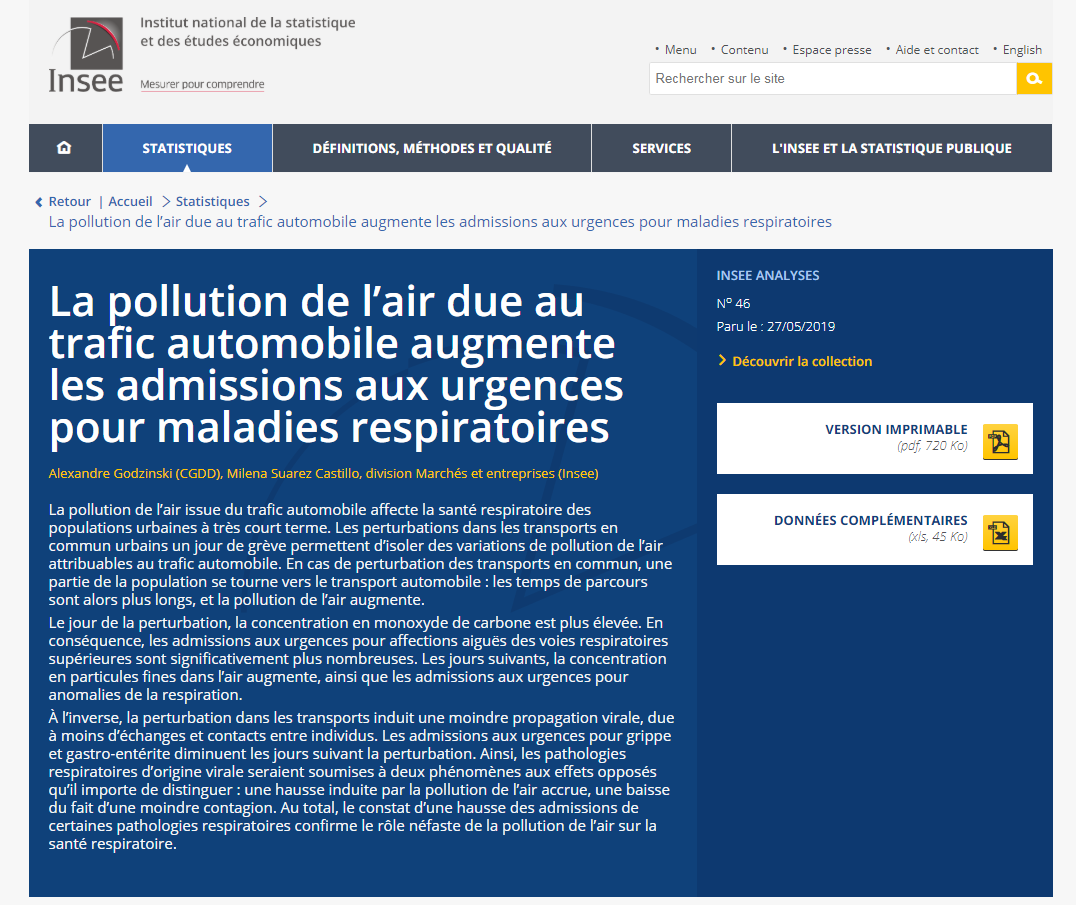
\includegraphics[scale=0.52]{images/insee-fr-exemple.png}
    \caption{Exemple de publication sur le site insee.fr}
    \label{fig:insee.fr}
\end{figure}

Les informations diffusées ont des formats divers~: tableaux, graphiques, cartes et fichiers détails accompagnent généralement les données textuelles des publications. Bien que le fichier structurant la publication soit toujours un fichier XML, le format des données textuelles est varié. Certains types de publications sont au format PDF texte, PDF image, PNG ou encore XLS lorsqu'il s'agit de tableaux. La plupart des publications où l'on retrouve du texte explicatif, du langage naturel, est présente en base de donnée sous format XML ; les différentes figures étant parfois traduites dans ce même format. Il sera donc aisé de sélectionner un corpus représentatif des publications. 
\newline

Voici un exemple de publication au format XML~: 

\begin{lstlisting}[language=XML, basicstyle=\small]
<?xml version="1.0" encoding="UTF-8" standalone="yes"?>
<publication-sans-sommaire afficher-sommaire="true"
                        afficher-sommaire-documentation="false">
	<titre>La pollution de l'air due au trafic automobile augmente 
	les admissions aux urgences pour maladies respiratoires</titre>
	<auteur>Alexandre Godzinski (CGDD), Milena Suarez Castillo, 
	division Marchés et entreprises (Insee)</auteur>
	<numero>46</numero>
	<chapo>
		<paragraphe>La pollution de l'air issue du trafic automobile [...]<paragraphe>
		<paragraphe>Le jour de la perturbation, la concentration [...]</paragraphe>
	</chapo>
	...
\end{lstlisting}

Un exemple complet est donné en annexe page \pageref{publication-xml}.
\newline

Certaines collections sont destinées à un public éclairé, comme les documents de travail ou la collection «~Economie et Statistique~», et le langage utilisé y est assez technique et parfois très spécifique. Dans la plupart des publications, un langage grand public est utilisé, avec toutefois le vocabulaire de la statistique, qui est celui qui nous intéresse ici. Les publications contiennent parfois des liens hypertextes vers les définitions des concepts statistiques mentionnées. Ces concepts sont dans leur entièreté nommés par leur libellé exact. Dans les cas ou ils ne contiennent pas de liens, le libellé est parfois incomplet ou enrichi par des adjectifs placés au milieu du libellé, rendant la reconnaissance plus ardue. Il y a quelques fois une ambiguïté sur le concept nommé, notamment pour ceux ayant des spécificités. Voilà quelques exemples de phrases faisant mention de certains concepts~:
\begin{itemize}
    \vspace{5pt}
    \item «~En 2018, l'activité des \textbf{secteurs commerciaux} est contrastée. Dans le \textbf{commerce de gros}, les ventes restent toniques (+ 1,9 \% en volume comme en 2017), en particulier dans le \textbf{commerce de biens d'équipement et de biens domestiques}.~», Insee Première 1759, 21/06/2019.
    Les libellés des concepts abordés sont «~Commerce~» et «~Commerce de gros~».
    \vspace{5pt}
    \item «~Fin 2017, le \textbf{patrimoine économique national net} s’élève à 14 762 milliards d’euros, soit 7,9 fois le \textbf{produit intérieur net} de l’année.~», Insee Première 1731, 17/01/2019.
    Les libellés des concepts abordés sont «~Patrimoine national~» et «~Produit intérieur net~».
\end{itemize}
\label{section 1.2.2}

\subsection{La Data science à l'Insee}

L'Insee jouit d'une situation particulière dans le domaine du \textit{Big Data} et des \textit{Data sciences}. Tout d'abord, en tant qu'institut d'envergure nationale, il dispose d'une culture du traitement de la donnée, et par conséquent d'une solide expérience sur les problématiques de qualité des données brutes. Cela est en effet l'une des étapes prenant le plus de temps dans les Data sciences~: la préparation des données.
\newline

L'institut dispose par ailleurs d'une légitimité et d'un droit d'exploitation des gisements de données de par son activité. Le Règlement Général sur la Protection des Données a contraint les entreprises à trouver d'autres moyens d'obtenir des données. Cela se traduit souvent par la génération en interne de données, parfois difficile.
\newline

L'Insee dispose enfin de compétences de haut niveau dans le domaine des statistiques, domaine connexe à celui de la Data science. J'ai d'ailleurs pu obtenir des aides précieuses, notamment dans l'explication des concepts ou encore dans l'utilisation de certains algorithmes.
\newline

\subsection*{Conclusion}
L'environnement que j'ai découvert et l'étude des données sur lesquelles j'ai été amené à travailler m'ont permis de mieux formaliser les rendus du stage.

L'objectif est de construire un premier service de reconnaissance d'entités nommées qui se focalise sur les concepts statistiques de la base RMéS dans les publications de l'Insee. Il s'agit également de fournir de la documentation sur le traitement du langage naturel et les principaux outils existants aujourd'hui.

\newpage
\section{La reconnaissance d'entités nommées~: découverte et enjeux}
N'ayant aucune connaissance préalable sur le traitement du langage naturel, ou NLP pour \textit{Natural Language Processing}, dont la reconnaissance d'entités nommées, ou NER pour \textit{Named Entity Recognition} fait partie, il faut adapter ma démarche. Tout d'abord en se documentant sur le sujet, puis en lisant des publications de recherche, afin de connaître l'état de l'art, et enfin en développant un premier service, pour en avoir une vision pratique. Cette démarche a été grandement facilitée par les moyens techniques mis à ma disposition.
\newline

\subsection{La reconnaissance d'entités nommées pour l'Insee}

\subsubsection{Le traitement du langage naturel}
Le traitement du langage naturel est un domaine qui s'attache, à partir d'un texte, à en analyser le sens et à en extraire une connaissance. Il permet par exemple d'analyser les sentiments dans un texte, ou encore à repérer les mentions d'organisations ou de personnes.
\newline

Il prend la forme d'un «~pipeline~», c'est-à-dire une succession de traitements, chacun donnant une information différente sur le texte. Parmi les traitements les plus courants on trouve~:
\begin{enumerate}
    \item \textit{Tokenisation}~: un pré-traitement qui permet de découper les textes en «~tokens~» à savoir en mots et éléments de ponctuation.
    \vspace{5pt}
    \item \textit{Sentence Split}~: un second pré-traitement qui permet de découper les textes en phrases ou propositions suivant les langues.
    \vspace{5pt}
    \item \textit{Part-of-speech tagging}~: un premier traitement donnant pour chaque token sa nature grammaticale (verbe, adjectif, nom, ponctuation, etc.)
    \vspace{5pt}
    \item \textit{Lemmatisation}~: un traitement souvent complémentaire au précédent, il s'attache à donner, pour chaque mot, l'entrée du dictionnaire de la langue correspondante. Pour un verbe conjugué par exemple, le lemme correspond à l'infinitif.
    \vspace{5pt}
    \item \textit{Dependencies}~: un traitement proposition par proposition, ou phrase par phrase, donnant les dépendances entre les mots. Par exemple quel adjectif est rattaché à quel nom, quel adverbe à quel verbe.
\end{enumerate}
\vspace{10pt}

\begin{figure}[H]
    \centering
    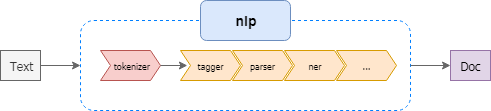
\includegraphics[scale=0.34]{images/Pipeline-example.png}
    \caption{Exemple de pipeline NLP}
    \label{fig:nlp-pipeline-example}
\end{figure}

\vspace{10pt}

On obtient en sortie de ce pipeline des informations à divers niveaux~: \textit{Part-of-speech tagging} et \textit{Lemmatisation} opèrent sur les mots, tandis que \textit{Dependencies} opère sur les phrases et propositions. D'autres traitements, tels que \textit{Coreference resolution} opèrent sur des textes; ce traitement permet de relier les pronoms et autres noms lorsqu'ils font référence à la même entité. Des exemples pour chaque traitement sont donnés en annexe page \pageref{nlp-exemple}.
\newline

Les différentes techniques du traitement du langage naturel, jusqu'alors peu généralisables, ont beaucoup évolué suite à l'arrivée des techniques à base de réseaux de neurones entre 2015 et 2017. C'est pourquoi ce domaine atteint aujourd'hui de meilleures performances, notamment en ce qui concerne la reconnaissance d'entités nommées. Les nouvelles techniques donnent des résultats plus précis, tout en gardant des temps de traitements équivalents aux techniques classiques.
\label{section 2.1.1}

\subsubsection{La reconnaissance d'entités nommées}

\subsubsection*{REN et Désambiguïsation}
La reconnaissance d'entités nommées est l'étiquetage dans un texte d'un mot ou d'un groupe de mots, ainsi que la classification de ce mot ou groupe de mots. Ces classes comprennent de façon générique les personnes, les dates, les lieux ou encore les organisations (instituts, associations, entreprises, etc.). Ce traitement inclut souvent un autre traitement que l'on appelle \textit{Entity Linking} ou \textit{Disambiguation}, qui est le fait de rattacher une occurrence d'entités nommées dans un texte à une base de connaissance, en utilisant le contexte. Prenons un exemple tiré d'\href{https://ambiversenlu.mpi-inf.mpg.de/}{Ambiverse NLU} \cite{ambiverse-nlu}, un service développé par l'Institut de recherche Max Planck effectuant ces deux traitements~:
\newline

\begin{figure}[H]
    \centering
    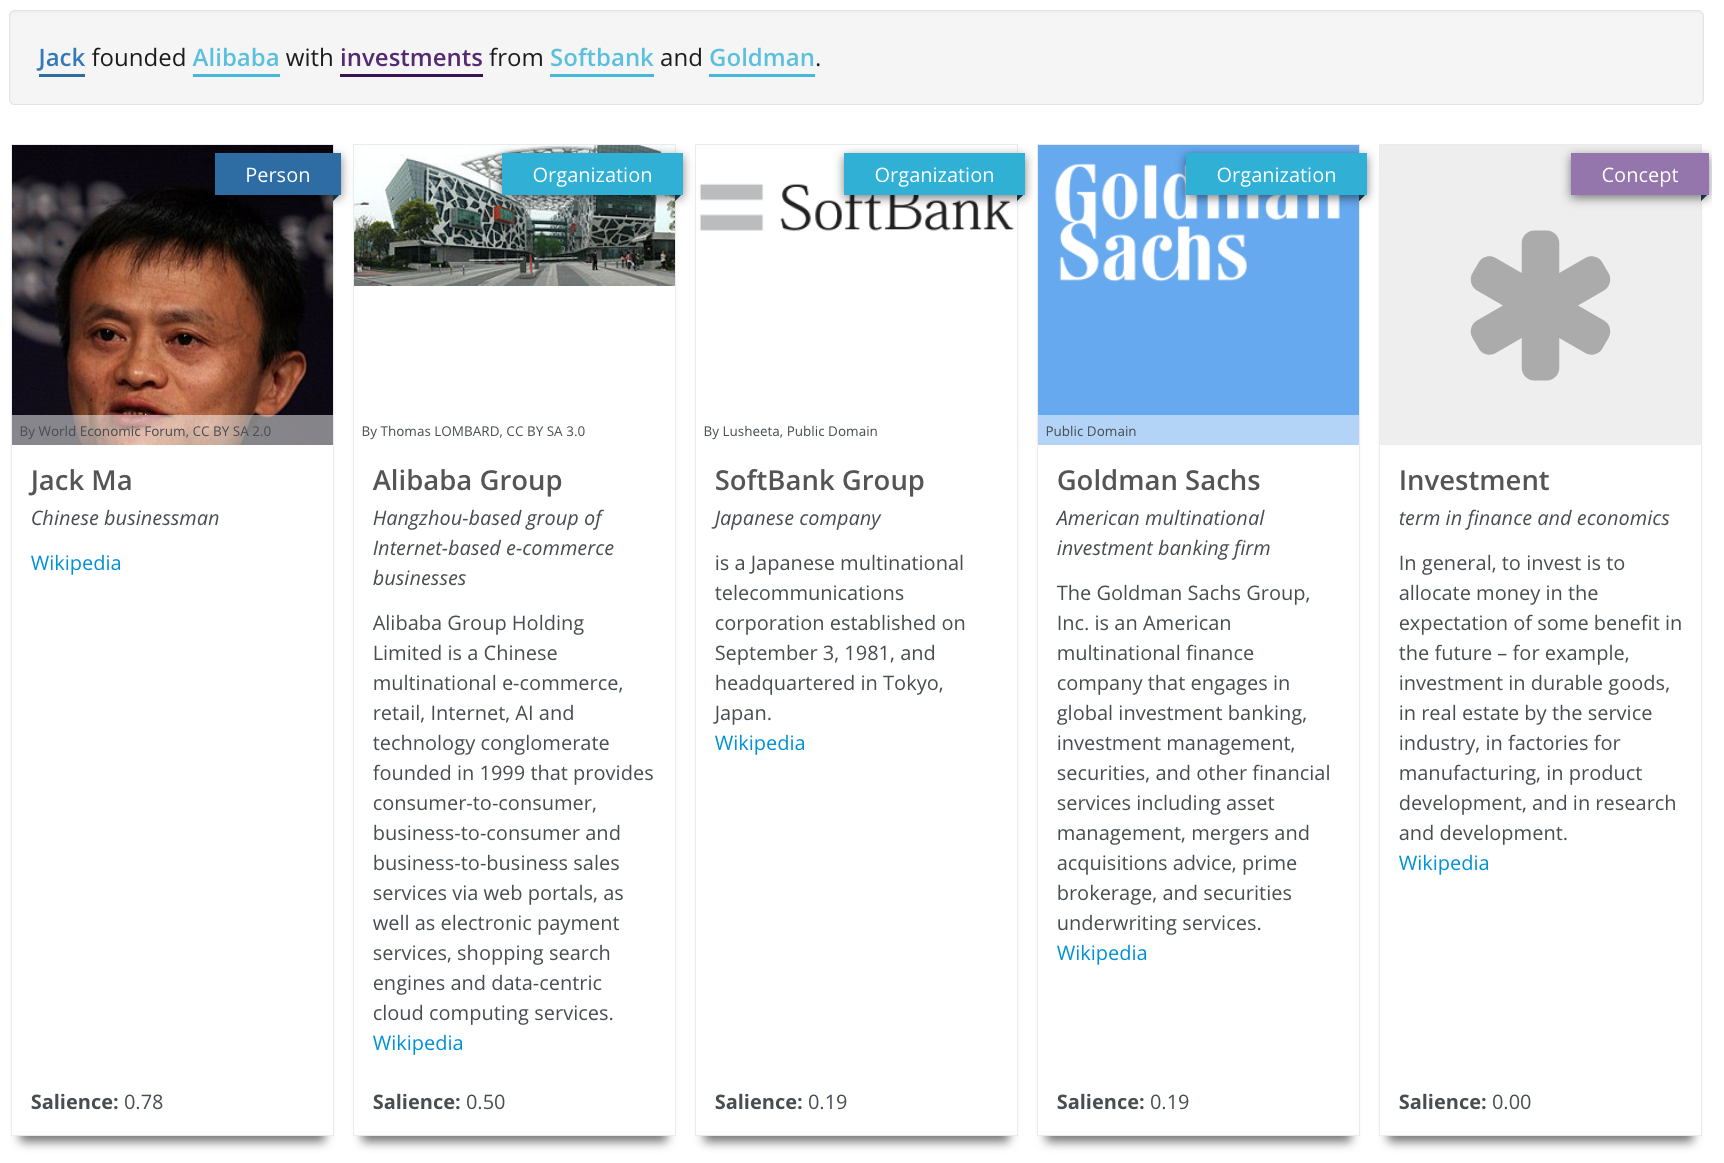
\includegraphics[scale=0.24]{images/ner-demo.png}
    \caption{Exemple de REN et de Désambiguisation}
    \label{fig:ner-demo}
\end{figure}

\vspace{10pt}

Dans la phrase d'exemple çi-dessus, la reconnaissance d'entités nommées à proprement parler est le fait d'étiqueter les quatre premiers caractères, c'est-à-dire le mot «~Jack~», comme faisant mention d'une personne. La désambiguïsation est le fait de lier le mot «~Jack~», dans le contexte de la phrase à Jack Ma. Dans le cas d'Ambiverse NLU, c'est la base donnée DBPedia, graphe RDF généré à partir des données de Wikipedia, qui est utilisée comme base de connaissance.
\newline

Dans la littérature, beaucoup s'interrogent sur la définition d'une entité, plus particulièrement sur les classes utilisées dans la reconnaissance d'entités nommées. Doit-on rester générique, en utilisant la classe «~personne~», laissant un travail de désambiguïsation plus conséquent ? Ou alors doit-on être plus spécifique en utilisant son statut (peintre, musicien, chef d'entreprise) ?

La question se pose également dans le cas des concepts statistiques. Le référentiel regroupe des entités diverses~: des entités géographiques (Commune, Département, Région, France hors Mayotte), une monnaie (Euro), des entités diverses (ADSL), des concepts juridiques ou statistiques (Coût salarial, Chômage) et même des entités dont la classe peut être ambiguë (Commune multipolarisée). La classification nécessite parfois une expertise de haut niveau sur la statistique, d'autant plus que ces classes n'apparaissent pas dans la base RMéS. Le choix provisoire est de tout rassembler sous la même classe «~concept statistique~», afin de se concentrer sur la REN à proprement parler.
\label{section 2.1.2 - REN et Désambiguïsation}

\subsubsection*{Les méthodes de reconnaissance d'entités nommées}
Pour effectuer la reconnaissance d'entités nommées, il existe deux méthodes~: 
\begin{enumerate}
    \item L'annotation à base de règles ou \textit{Rule based matching}~: elle permet d'annoter de manière déterministe les mots ou groupes de mots validant une règle. Cette règle peut porter sur les simples chaînes de caractères (expression régulière) ou sur les résultats du traitement du langage naturel (\textit{Part-of-speech}, \textit{Lemmatisation}, etc.). On peut par exemple établir une règle qui cherche toute occurrence d'un mot ayant pour lemme «~salaire~» et étant suivi de deux adjectifs. Ainsi, dans la phrase~: «~le salaire net moyen augmente de 1,1 \% en euros constants par rapport à 2014~», la règle étiquetterait «~salaire net moyen~». D'autres exemples de règles ainsi que leur résultat sont donnés en annexe page \pageref{rule-exemple}.
    \vspace{5pt}
    \item L'annotation à base d'apprentissage~: la méthode consiste à entraîner un réseau de neurones sur des données d'exemples. Il existe différentes architectures de réseaux de neurones pour effectuer de la REN. \href{https://www.aclweb.org/anthology/Q16-1026}{Ciu et Nichols} \cite{chiu-nichols}, \href{https://www.aclweb.org/anthology/N16-1030}{Lample et. al} \cite{lampe-al}, et d'autres ont tous en commun certains éléments. Le principe est d'analyser les phrases mot à mot~: pour chacun d'entre eux, on calcule et stocke un vecteur, qui va servir au réseau attribuant un label. Cette méthode de «~stockage~» est appelé LSTM, pour \textit{Long short-term Memory}. D'autres résultats du TLN, comme le tag \textit{Part-of-Speech} sont parfois stockés à l'aide de la méthode LSTM. Ces données sont ensuite traitées par un autre réseau qui détermine le libellé d'entité nommée. Des références sont données dans la bibliographie.
    \newline
\end{enumerate}

L'avantage de la première méthode est qu'elle ne nécessite aucun pré-requis, et qu'elle permet de faire la désambiguïsation plus aisément en associant pour chaque règle un identifiant. Cependant elle ne permet pas de généralisation, c'est-à-dire l'annotation d'entités inconnues, contrairement à la deuxième méthode. C'est en effet le point fort des méthodes à base de réseaux de neurone, qui nécessitent néanmoins de disposer de données d'apprentissage. Dans le cas de la reconnaissance d'entités nommées, ces données sont des textes dont les mots représentant les entités nommées sont repérés. Il existe cependant plusieurs prérequis sur les données d'apprentissage~:
\newline

Tout d'abord le volume des données~: il doit être suffisant pour que tous les cas de figure soient représentés, et si possible dans les bonnes proportions. Dans le cas de la reconnaissance d'entités nommées, il est difficile de définir la représentativité des données. Il faut évidemment que les concepts soient tous cités un certain nombre de fois dans le corpus des données. En revanche, définir les cas de figure est très expérimental. Prenons le cas du concept intitulé «~Solde apparent des entrées sorties~»~: il faut tout d'abord analyser sous quelles formes il est cité dans les publications. On trouve parfois «~solde des entrées sorties~», quand il est déjà cité avec son libellé complet dans le texte. La question de la représentativité est de savoir quelle est la proportion d'occurrence de cette forme du concept dans le corpus d'entraînement, et est donc spécifique à chaque concept, et peut-être même aux langages utilisés dans les publications. Suivant que le langage utilisé soit très technique, comme on le retrouve dans certaines publications, ou courant, les termes utilisés pour désigner les concepts sont différents.
\newline

On retrouve dans les textes de la plupart des publications de l'Insee des liens vers les concepts et leurs définitions, ces derniers pouvant servir de base d'apprentissage. Cependant ils ne sont pas suffisamment nombreux pour être représentatif de tous les cas rencontrés. C'est pourquoi le choix s'est rapidement porté sur l'annotation à base de règles.
\newline

L'hypothèse à plus long terme de se constituer une base d'apprentissage n'est cependant pas écartée. Le premier outil développé pourrait permettre, à l'aide une correction manuelle apportée par les rédacteurs quand cela est nécessaire, de se constituer cette base.
\label{section 2.1.2 - Méthodes de REN}

\subsubsection{Une première utilisation~: amélioration de la qualité des publications}
Comme mentionné dans la partie \ref{section 1.2.2}, l'objectif principal d'un tel service est d'améliorer les publications. Plus précisément, il s'agit de donner un retour aux auteurs des publications sur les concepts mentionnés dans leurs écrits. 
\newline

Le premier cas d'application serait en effet d'avertir les auteurs sur les concepts statistiques employés dans une publication, afin d'en retirer l'éventuelle ambiguïté sur le terme cité. Par exemple, le concept de «~population active~» a un sens légèrement différent suivant si on l'entend au sens du Bureau International du Travail (BIT) ou au sens du recensement. Le service pourrait servir à alerter l'auteur si l'on ne peut déterminer, à partir d'informations figurant dans la publication, s'il s'agit de la population active au sens du BIT ou au sens du recensement.
\newline

De plus, comme vu dans la section \ref{section 1.2.1}, le référentiel des méta-données statistiques n'est pas complet. Un cas d'utilisation de la reconnaissance d'entités nommées est donc, pour un auteur, une occasion de vérifier si le concept utilisé figure dans le référentiel. Ainsi, un tel service pourrait favoriser un travail collaboratif autour du référentiel, et ainsi permettre de le compléter.
\newline

C'est donc avec ce premier objectif en tête que je pense le service~: permettre à un utilisateur de soumettre une publication pour voir quels sont les concepts qui sont reconnus et à quelles entrées de la base RMéS ils sont rattachés.
\label{section 2.1.3}

\subsubsection{Les champs d'application à long terme}
Sur le long terme, un tel service pourrait également servir à automatiser certaines tâches, toujours dans le cadre de la diffusion de l'information.
\newline

La première application est assez naturellement l'insertion de liens hypertextes vers les définitions des concepts repérés. Cela faciliterait le travail des rédacteurs. 
\newline

Un tel outil peut aussi servir à effectuer de l'indexation de contenu sur les publications de l'Insee. Elle est aujourd'hui effectuée à partir du moteur de recherche \textbf{Solr}, qui indexe les contenus par rapport au vocabulaire utilisé dans le titre, le sous-titre et le chapô des publications. À moins que le concept soit mentionné de manière exacte dans l'un de ses trois éléments, la publication n'est pas indexée par rapport au concept. Avec l'outil, on pourrait affiner l'indexation effectuée par Solr, et ainsi permettre aux utilisateurs de soumettre des recherches plus précises. Explorer les possibilités d'indexation vis-à-vis des concepts retrouvés dans les publications est donc envisageable mais ne répond pour le moment pas à un besoin de l'Insee.
\newline

D'autres organismes se montrent intéressés par le projet ainsi qu'à la reconnaissance d'entités nommées en général~: \textbf{Eurostat}, qui est l'organisme coordonnant les actions des instituts nationaux de statistique, se montre intéressé par le projet. Le Ministère de la Justice aimerait également étudier les possibilités offertes par le traitement du langage naturel pour rendre anonymes certains documents.
\newline

La diversité des champs d'application d'un service de reconnaissance d'entités nommées nécessite une réflexion approfondie sur l'architecture du service, architecture qui est décrite partie \ref{section 3.2.1 - Architecture des services}. Cela implique également d'adopter une méthode de travail agile. Les fonctionnalités offertes par le traitement du langage naturel ainsi que les données en libre accès (\textit{Linked Open Data}) évoluent en permanence et il est probable qu'un tel service soit également amené à beaucoup évoluer.
\label{section 2.1.4}

\subsection{Une première implémentation facilitée par la plateforme}

\subsubsection{La plateforme innovation}
Travaillant à la DIIT (voir section \ref{section 1.1.2}), j'ai la chance d'évoluer au plus près de la plateforme Innovation. Cette plateforme a pour but de mettre à disposition de tous les agents Insee un environnement pour prototyper, tester et découvrir des nouveaux services. Elle est en quelque sorte un «~bac à sable~» pour les développeurs et les statisticiens, et une plateforme de travail collaborative pour les agents Insee. Maintenu par la DIIT, c'est un projet en développement et ne doit par conséquent pas être confondue avec les services actuellement maintenus en production. Elle m'offre d'une part une vision très pratique de ce qui m'a été enseigné dans ma voie d'approfondissement, et d'autre part un environnement de développement idéal pour la tâche qui m'est confiée.
\newline

Son implémentation est fondée sur une architecture CaaS, \textit{Container as a Service}. La disponibilité est de type \textit{Best effort}~: cela signifie que les garanties de services sont limitées. La fraîcheur des mises à jour et des derniers standards techniques est préféré à la stabilité et au maintien des services. La confidentialité n'est pas garantie, ce qui implique qu'aucune donnée sensible ne doit y être déposée.
\newline

Les données sur lesquelles je travaille sont disponibles sur le web, et ne sont donc pas confidentielles. Cette plateforme m'offre des outils tout à fait adaptés à mon projet de stage, comme à mon projet professionnel. L'administration de plateforme \textit{CaaS} fait en effet partie des métiers qui m'intéressent. Découvrir les aspects techniques et humains d'une telle activité à été pour moi très enrichissant.
\label{section 2.2.1}

\subsubsection*{Architecture}
\vspace{10pt}
\begin{figure}[H]
  \centering
  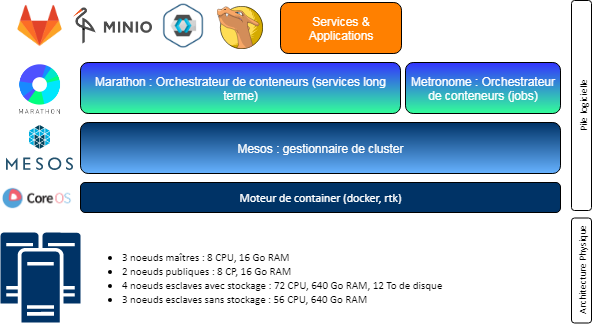
\includegraphics[scale=0.70]{images/Archi-inno.png}
  \caption{Architecture simplifiée de la plateforme Innovation}
  \label{fig:une-image}
\end{figure}
\vspace{10pt}

L'architecture physique totalise pour la gestion d'application 456 CPU, 4480 Go de RAM et 48 To de stockage disque. Côté logiciel, il s'agit d'un cluster \textbf{Mesos} utilisant \textbf{Marathon} et \textbf{Metronome} comme orchestrateur de conteneurs, accompagnés de plusieurs services longues durées (de gauche à droite sur le schéma):
\begin{enumerate}
    \item \href{https://about.gitlab.com/}{\textbf{Gitlab}} \cite{gitlab}~: la forge logicielle de la plateforme. Elle est dotée notamment d'un CI/CD (\textit{Continuous Integration / Continuous Delivery}), facilitant la mise à jour des services de la plateforme. La configuration des services de longue durée y est stockée~: chaque service longue durée a un projet Gitlab qui lui est associé, exception faite des services centraux (Gitlab, Minio). Les Gitlab-runners de la plateforme permettent, via Gitlab, de mettre à jour les services de la plateforme et d'en déployer de nouveaux en sollicitant l'API Marathon.
    \vspace{5pt}
    \item \href{https://min.io/}{\textbf{Minio}} \cite{minio}~: service de stockage réparti orienté objet. Minio est une implémentation de S3, \textit{Simple Storage System}, développé par \textbf{Amazon}. Il offre par conséquent une API compatible avec beaucoup de clients, en plus d'une interface Web pour gérer ses fichiers à la main.
    \vspace{5pt}
    \item \href{https://www.keycloak.org/}{\textbf{KeyCloak}} \cite{keycloak}~: service d'authentification et de gestion d'accès. Il fournit aux services une API pour gérer l'authentification. Il est notamment utilisé par Gitlab et par Minio (session).
    \vspace{5pt}
    \item \textbf{Onyxia}~: service web d'utilisation de la plateforme. Développé en interne, il regroupe une IHM et une API. L'IHM, portail d'entrée pour les utilisateurs de la plateforme, fournit la liste des services longues durées de la plateforme, une liste d'applications dites «~self~», que chacun peut lancer (des IDEs, outils bureautiques, etc.) ainsi qu'une IHM pour interagir avec Minio (déposer des fichiers par exemple). Afin de lancer un self-service, elle communique avec l'API REST Onyxia. Cette dernière dialogue avec Marathon et Mesos pour lancer le conteneur et ouvrir l'accès à l'utilisateur.
    \vspace{5pt}
    \item Et beaucoup d'autres applications ! \href{https://www.vaultproject.io/}{\textbf{Vault}} \cite{vault}, gestionnaire de secrets, \href{https://fr.sonatype.com/nexus-repository-sonatype}{\textbf{Nexus}} \cite{nexus}, gestionnaire de dépôt, \href{https://rocket.chat/}{\textbf{RocketChat}} \cite{rocketchat}, serveur de messagerie instantanée ou encore \href{https://humhub.org}{\textbf{Humhub}} \cite{humhub}, réseau social d'entreprise sont déployés sur Marathon.
    \newline
\end{enumerate}

La plateforme fournit également des services à la demande, ou self-services. La majorité d'entre eux est orientée développement ou statistique, mais certains sont des outils collaboratifs à la destination de tous. Elle totalise donc une soixantaine de services. Dans la continuité des missions de la DIIT, le but de la plateforme est également d'encourager le travail collaboratif, notamment autour de la gestion et l'entretien des services mis à disposition.

\subsubsection{Une approche collaborative}
Je découvre tout au long du stage un fonctionnement humain centré sur la collaboration et l'ouverture. Bien que celui-ci me soit familier de par mon engagement associatif à l'école, je l'observe à l'Insee sous une toute autre échelle et avec une diversité des profils. Certains services sont en effet maintenus aujourd'hui par des statisticiens, qui ont en général une vision pratique, une vision métier de l'informatique. Cela a été rendu possible par les incubations qu'offre la DIIT.
\newline

Ces incubations, auxquelles j'ai pu participer, durent deux ou trois jours. Elles ont pour but d'aider une équipe sur leur projet de développement. L'équipe vient avec une problématique technique relative aux méthodes de développement DevOps. Le but est de leur donner les outils et compétences pour être à même d'intégrer cette démarche~: elle inclut en général un apprentissage de \textbf{Git} lorsque cela est nécessaire, et plus souvent le fonctionnement de Gitlab-CI, de \textbf{Docker} et de Marathon. J'ai la chance lors de ces incubations d'en apprendre davantage sur la plateforme en explorant les différents cas d'usage, mais aussi en apportant mon aide aux incubés concernant l'utilisation de Git et de Docker par exemple. C'est ainsi que la DIIT favorise une gestion commune de la plateforme, les incubations aboutissant parfois au déploiement d'un nouveau service sur la plateforme, service géré principalement par l'équipe incubée. Suite à une incubation, deux statisticiens des bureaux de Marseille gèrent aujourd'hui un service \textit{OpenStreetMap} sur la plateforme, qui leur permet d'effectuer des statistiques sur les temps de trajet entre domicile et travail à partir des données du recensement.
\newline

Travaillant sur les environnements de développement disponibles en self-service, j'ai également contribué au projet \textbf{Desktop Ubuntu} de la plateforme. Ce service permet de développer simplement sous un Ubuntu web, notamment en Java. Pour plus de confort et d'efficacité dans le développement, je contribue à l'image Docker Ubuntu proposé, en mettant à jour les IDEs et en y ajoutant certains plugins et paquets.
\label{section 2.2.2}

\subsubsection*{Le séminaire du développement}
Les échanges sur les nouveaux projets et technologies utilisées sont favorisés par un évènement qui a lieu chaque année et auquel j'ai eu la chance de participer~: le séminaire du développement. Pendant une semaine, chaque équipe de développement de l'Insee, incluant des équipes à Nantes, Lille et Orléans, a l'occasion de présenter à tous les développeurs les utilisations de nouvelles technologies dans leurs travaux.
\newline

Ce séminaire a été l'occasion pour moi de voir beaucoup de technologies et bibliothèques récentes en application concrète dans des projets. Écriture de grammaire avec \textbf{Antlr4}, automatisation de tests d'interface Web avec \textbf{Selenium} et \textbf{Cypress}, ou encore packaging d'applications Python pour du web avec \textbf{Flask}, le séminaire offre une bonne vue d'ensemble des technologies à l'oeuvre à l'Insee. J'ai moi aussi eu l'occasion de présenter mes premiers résultats sur l'utilisation du traitement du langage naturel dans les publications de l'institut. Des échanges sur les différentes bibliothèques existantes me permettent de mettre à l'épreuve le premier pipeline construit, et ainsi de l'améliorer.
\newline

La démarche participative de la plateforme est favorisée jusque dans les salles serveurs ! Avec l'arrivée de quatre nouvelles machines, j'ai apporté mon aide pour remplacer les noeuds esclaves de stockage de la plateforme innovation. Au programme~: câblage, configuration réseau et installation de système d'exploitation. 

\begin{figure}[H]
    \centering
    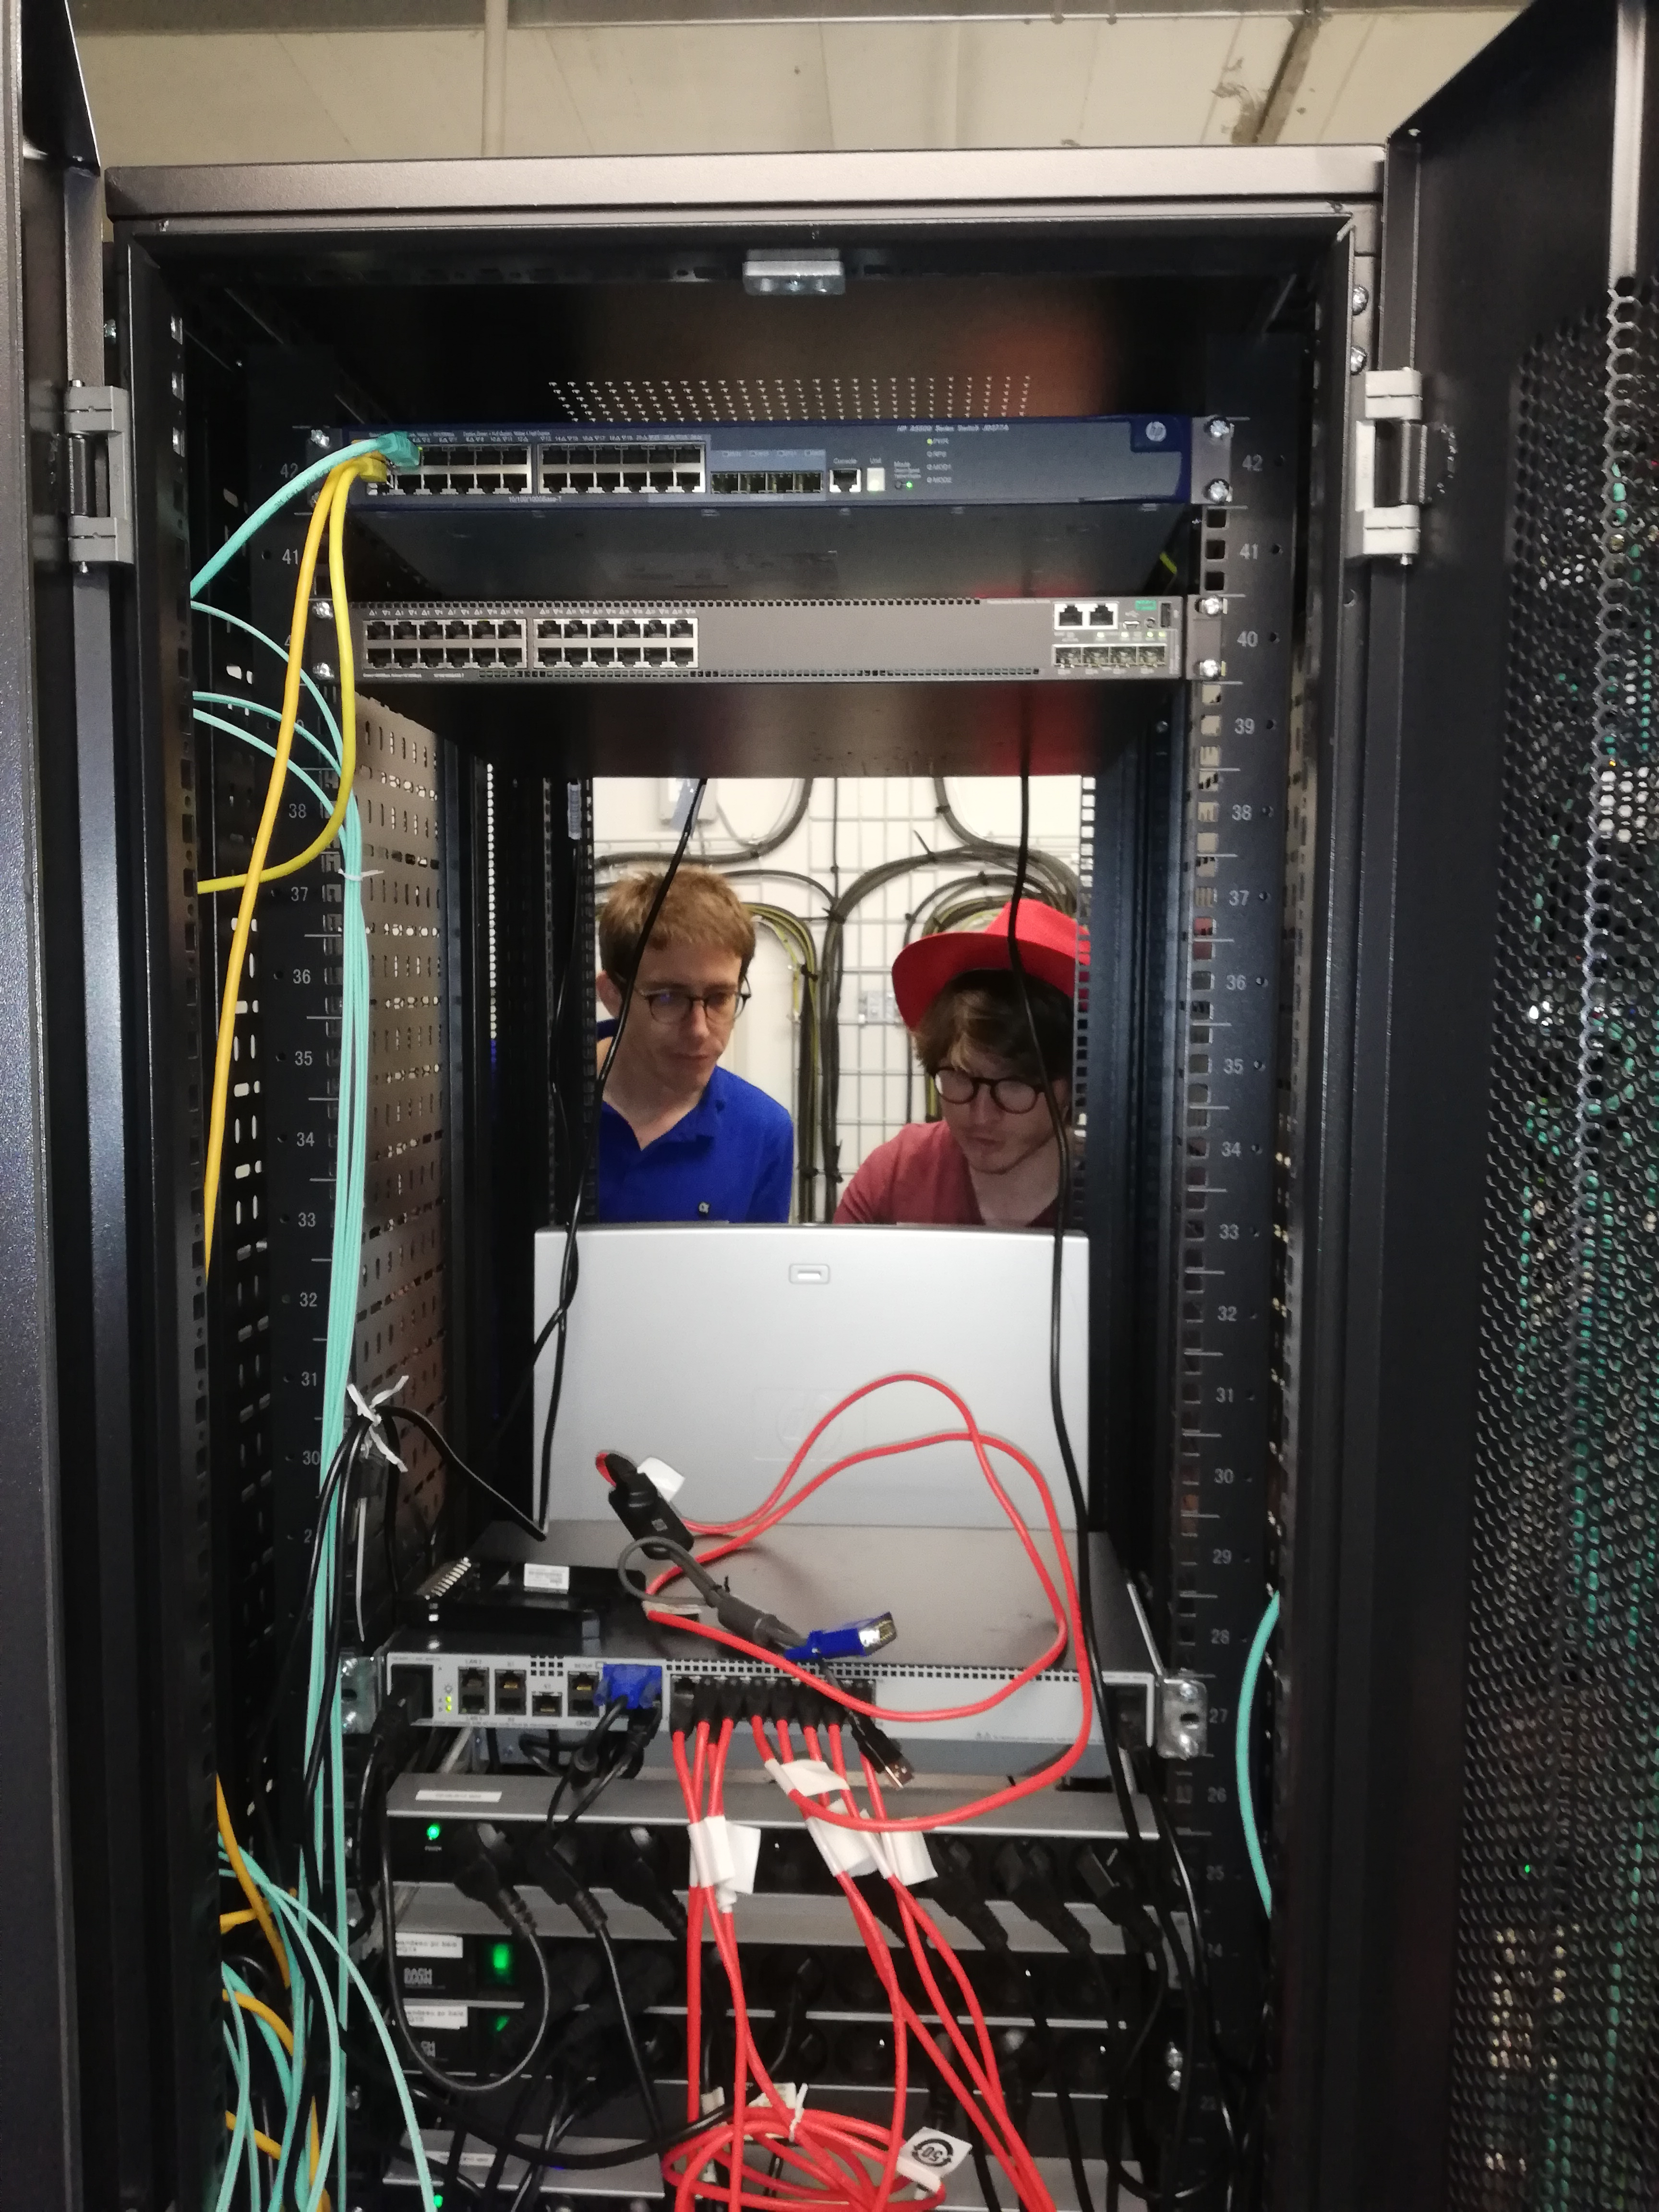
\includegraphics[scale=0.10]{images/salle-machine.jpg}
    \caption{Frédéric Comte (à gauche) et moi-même (à droite) en salle machine}
    \label{fig:salle-machine}
\end{figure}
\vspace{10pt}

C'est dans cette démarche collaborative autour du développement que j'ai d'une part adopté la pratique DevOps et d'autre part aidé des agents Insee autour de cette pratique.
\label{section 2.2.2 - Séminaire du développement}

\subsubsection{La pratique DevOps}
La pratique DevOps est le fait de développer un projet de manière continue, du développement du logiciel cœur jusqu'à sa livraison et sa maintenance pour l'utilisateur final. Souvent accompagné d'une démarche agile, il s'agit dans cette méthode d'assurer et de suivre toutes les étapes de vie d'un logiciel~: développer, intégrer, tester, déployer, exploiter et maintenir les fonctionnalités d'une application de manière continue. Le principe est de faire des cycles de développement courts, et des livraisons fréquentes, afin de mieux s'adapter aux changements. L'automatisation de certaines tâches, comme le déploiement ou les tests, fait pleinement partie de cette démarche.
\newline

La plateforme, avec \textbf{GitLab-CI/CD}, \textbf{Nexus} et l'API \textbf{Onyxia}, offre tous les outils pour adopter la démarche. Pour mon premier pipeline réalisé en Java et utilisant le gestionnaire de dépendances \textbf{Maven}, j'ai pu mettre en place un pipeline GitLab qui teste mon application dans un environnement proche d'un environnement de production. C'est en effet l'un des avantages du DevOps~: préparer le terrain le plus en amont possible pour un passage en production. Le but n'est pas que de déployer une application fonctionnelle, mais de détecter les points d'amélioration sur le code existant. 
\newline

Pour la première maquette de mon application, il s'agit simplement de créer un pipeline GitLab permettant d'exécuter du code Java. Concrètement, cela se présente sous la forme d'un fichier, \textit{.gitlab-ci.yml}, qui spécifie les étapes de mon pipeline. Chaque étape correspond au déploiement d'un conteneur Docker sur la plateforme, dont l'image utilisée est spécifiée dans le fichier. Dans notre cas, l'image utilisée inclue le JDK-8 (Java 8) ainsi que le gestionnaire de dépendances Maven. Il suffit ensuite d'indiquer les lignes de commande shell à exécuter pour effectuer les tests. Pour un projet fait avec \textbf{Maven}, les commandes à exécuter sont simples. La récupération des données l'est moins~: en effet, Gitlab ne publie par défaut que la sortie standard et la sortie d'erreur du conteneur. Dans le cas d'un déploiement, il est parfois nécessaire de conserver des fichiers écrits par l'application dans le conteneur. Nous y reviendrons dans la partie \ref{section 3.2.3} pour la description de la deuxième version du service.
\label{section 2.2.3}

\subsubsection{Les différentes méthodes testées}
Les premiers tests sur les méthodes de REN à base de règles ont été réalisés avec la bibliothèque \href{https://stanfordnlp.github.io/CoreNLP/}{Stanford Core NLP} \cite{corenlp-doc}. Ce choix a été guidé par l'orientation recherche de la bibliothèque~: l'intégration des dernières avancées techniques dans le TLN est préférée à la stabilité. C'est en effet parmi les premières à proposer en 2015 des traitements basés sur le \textit{Deep Learning}. Écrite en Java, elle me permet en plus de concentrer mes efforts sur la méthode de REN et non sur l'implémentation. 
\newline

J'ai d'abord travaillé sur la reconnaissance des concepts statistiques à partir de leur libellé. Ces derniers ont diverses formes, avec parfois des annotations qu'on ne retrouve pas dans les publications. J'ai donc éliminé pour les tests les concepts dont les libellés ont des parenthèses et les longs libellés avec énumération, ce qui laisse environ 700 concepts. Une difficulté majeure pour tester les méthodes de reconnaissance est l'obtention de données de tests fiables et représentatives~: d'une part, bien que la majorité des mentions de concepts statistiques soit aisée à repérer, certains utilisant des mots très communs ne le sont pas pour des non-spécialistes. D'autre part, les publications traitent généralement d'un sujet précis. Une publication ne sollicite finalement que peu de concepts statistiques, une dizaine en général. Il est donc difficile d'estimer la pertinence d'une méthode et c'est pourquoi je me suis attaché dans ces tests à reconnaître les groupes de mots pouvant être une occurrence de concept statistique. Les deux publications utilisées pour les tests sont tirées de la même collection~: \href{https://insee.fr/fr/statistiques/4129807}{Insee Première 1750} et \href{https://insee.fr/fr/statistiques/3703745}{Insee Première 1734}.
\newline

La toute première méthode testée est la plus triviale~: reconnaître les occurrences en faisant une simple recherche textuelle. Cette simple méthode permet déjà de trouver beaucoup d'occurrences de concepts, souvent ceux ayant des libellés courts et simples, comme «~salaire~» ou «~commune~». Pour identifier les autres occurrences, plusieurs outils de TLN peuvent être utilisés~:
\newline

\begin{itemize}
    \item \textit{Lemmatization}~: c'est le premier traitement à tester. La méthode utilisant la lemmatisation consiste à créer des règles indiquant des suites de lemmes, par exemple~: «~Toutes les suites de quatre tokens consécutifs ayant respectivement pour lemme \textit{petit}, \textit{et}, \textit{moyen}, et \textit{entreprise}~». Cela permet de s'affranchir du contexte grammatical~: qu'il soit cité au singulier comme dans le libellé, ou au pluriel, qui est la forme la plus couramment utilisée dans les publications, la règle utilisant les lemmes permet d'étiqueter le concept. Il est difficile d'effectuer le test avec Core NLP, la bibliothèque ne fournissant pas de lemmatisation pour le français. La bibliothèque fournit une interface permettant de créer son propre lemmatiseur. À l'aide d'un dictionnaire de lemmes, mis en ligne par \textit{Europeana} et disponible sur \href{http://www.iramuteq.org/}{Iramuteq} \cite{iramuteq}, j'ai construit mon propre lemmatiseur. Le principe est simplement d'associer à chaque mot son lemme. Sur les deux publications testées, l'implémentation de la méthode a permis de repérer plus de 120 occurrences dans chaque texte.
    \newline
    
    \item \textit{Part-of-Speech}~: l'idée derrière l'utilisation de ce traitement est d'améliorer la méthode décrite précédemment. La quasi-totalité des mentions de concepts dans les publications sont des groupes nominaux. Le nom principal est généralement présent mais les qualificatifs ne correspondent pas toujours à ceux utilisés dans les libellés~: il y en a parfois davantage, modifiant le libellé, parfois moins, les autres qualificatifs étant sous-entendus et dépendant souvent du contexte. «~salaire net moyen en EQTP~» fait par exemple référence à «~salaire en équivalent temps plein~». L'idée est donc de construire des règles comme celle-ci~: «~Tous les groupes nominaux dont le nom principal a pour lemme \textit{entreprise} dont au moins deux adjectifs ont pour lemmes \textit{petit} et \textit{moyen}~». Les tests sont plutôt concluants~: 177 concepts sont repérés dans la première publication et 181 dans la seconde.
    \newline
\end{itemize}

Les premiers tests sont encourageants mais ne couvrent qu'une petite partie des concepts de la base. Les règles sont de plus écrites à la main pour les quelques concepts testés. Pour passer à une plus grande échelle, j'ai construit un premier service de REN, incluant un générateur de règles.
\label{section 2.2.4}

\subsubsection{Premier service de REN}
Le premier service de reconnaissance d'entités nommées est construit avec la bibliothèque Stanford Core NLP. Afin qu'il soit modifiable et puisse aisément s'intégrer dans un pipeline GitLab-CI, l'architecture suivante est adoptée~:

\begin{figure}[H]
    \centering
    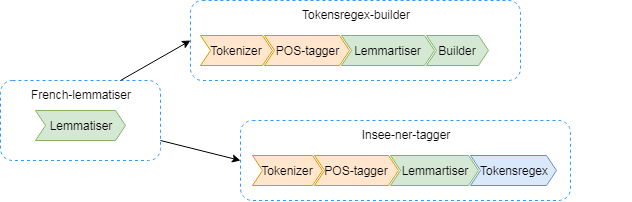
\includegraphics[scale=0.38]{images/Concept-tagger.png}
    \caption{Schéma fonctionnel du premier service de REN}
    \label{fig:premier-pipeline}
\end{figure}
\vspace{10pt}

L'architecture du service se décompose en trois modules~: 
\begin{itemize}
    \item \textit{French-lemmatiser}~: un module contenant la classe \textit{French-lemmatiser} et le dictionnaire de lemmes. C'est le composant associant à chaque token un lemme. La séparation du lemmatiseur en un seul module est un choix guidé par une exigence d'adaptabilité du code. La méthode de génération de règles doit être valable pour plusieurs langues, et le lemmatiseur est un composant spécifique à la langue. C'est pourquoi séparer ce composant en en faisant un module permet de passer facilement d'une langue à une autre.
    \vspace{5pt}
    \item \textit{Tokensregex-builder}~: il s'agit du générateur de règles, appelé «~ Tokensregex~» dans la bibliothèque Stanford Core NLP. Il prend en entrée une liste de groupes nominaux représentant des entités nommées et génère un fichier de règles au format spécifié par la bibliothèque. Elles sont générées en faisant tourner un pipeline Stanford Core NLP ayant les quatre composants décrits ci-dessus. Le composant \textit{Builder} prend en entrée les libellés annotés et donne en sortie des règles suivant ce schéma~: 
    \vspace{10pt}
    \begin{figure}[H]
        \centering
        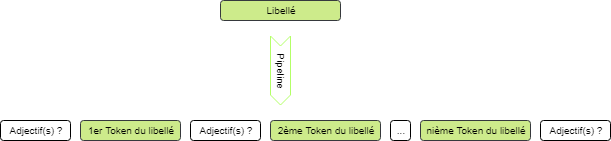
\includegraphics[scale=0.6]{images/Exemple-tokensregex.png}
        \caption{Schéma du construction d'une \textit{Tokensregex}}
        \label{fig:schema-tokensregex}
    \end{figure}
    \vspace{10pt}
    La sous-règle «~[1er, 2e, ...n]ième Token du libellé~» repère un token ayant le même lemme et la même nature grammaticale que le token du libellé. Cette fonctionnalité a été séparée en un module dans une volonté de produire du code réutilisable. Il n'est d'une part pas spécifique à l'Insee, et d'autre part il pourrait s'appliquer à d'autres langues.
    \vspace{5pt}
    \item \textit{Insee-ner-tagger}~: le module spécifique à l'Insee qui intègre le pipeline qui va traiter le texte des publications. Il contient deux classes~: la première est le pipeline Stanford Core NLP configuré pour reconnaître les concepts statistiques. Le fichier de sortie de \textit{Tokensregex-builder}, fichier de règles, figure parmi les ressources et est lu par le composant \textit{Tokensregex} qui annote le texte en fonction. La seconde classe gère le format XML des publications. Elle consiste en un processeur XSLT (langage de manipulation de fichiers XML), et en une feuille de style XSLT appelant le pipeline sur le contenu des balises désirées.
    \newline
\end{itemize}

Les interfaces sont conçues dans un souci de testabilité~: un autre module de test vient compléter cette liste. Ce dernier assure simplement la communication avec les différentes bases de données pour obtenir les publications souhaitées et ainsi tester le pipeline. Un client PostgreSQL permet d'obtenir les métadonnées sur les publications (leur type, la langue d'écriture, leurs identifiants, etc.), et permet d'obtenir les identifiants des publications que l'on peut obtenir via un serveur HTTP. Ces deux clients nous donnent les publications au format XML, et le programme principal le même fichier enrichi de balises XML repérant les occurrences de concepts. Pour plus de lisibilité lors de la vérification des concepts matchés, le module de texte inclut une seconde transformation XSLT afin d'obtenir un rendu HTML.
\newline

Mon pipeline de test se présente comme suit~:
\vspace{10pt}
\begin{figure}[H]
    \centering
    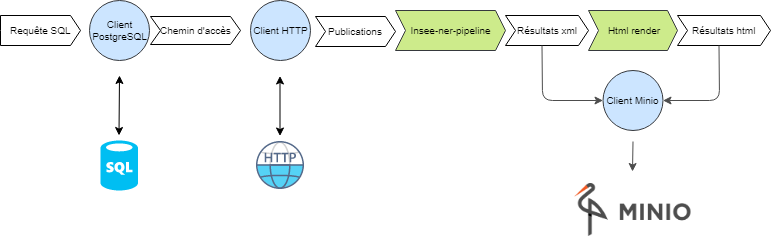
\includegraphics[scale=0.56]{images/Pipeline-test.png}
    \caption{Schéma du pipeline de test du service}
    \label{fig:pipeline-test}
\end{figure}
\vspace{10pt}

Il est lancé à chaque mise à jour du dépôt Git central, sur n'importe quelle branche, et enregistre les résultats sous format XML et HTML dans Minio.
\newline

\subsubsection*{Résultats à grande échelle}
Le pipeline est testé sur les publications \textit{Insee Première}, collection rassemblant des publications riches en données textuelles. Une rapide analyse statistique sur la couverture des concepts mentionnés ainsi que sur leur fréquence d'apparition révèle certaines lacunes du pipeline. Trois sont décrites ci-dessous.
\newline

Premièrement, la lemmatisation est lacunaire~: en effet, la connaissance seule de l'orthographe d'un mot ne suffit pas à donner le mot du dictionnaire associé. Par exemple, le mot «~moyen~» peut correspondre à l'adjectif ou bien au nom. C'est pour cela que le concept «~petite et moyenne entreprise~» n'est jamais reconnu~: «~moyenne~» est lemmatisée en le nom «~moyenne~», désignant la moyenne statistique, tandis que le mot «~moyennes~» est lemmatisé en l'adjectif «~moyen~» dans le dictionnaire de lemmes utilisés. Ce dernier n'est d'ailleurs pas complet et ne propose pas de lemme pour certains mots peu fréquents tels que «~multipolarisé~». Une solution est de ne pas utiliser seulement l'orthographe du mot pour trouver son lemme, mais également sa nature grammaticale. Cette solution n'est pas simple à mettre en oeuvre. Il s'agit de trouver ou générer un dictionnaire < < mot, nature >, lemme >.
\newline

Deuxièmement, la tokenization est destructive~: cette étape permet de découper le texte en mots et éléments de ponctuation. Dans la plupart des cas cela est simple. Les quelques exceptions sont les contractions de certains mots, comme «~de~» et «~le~» contracté en «~du~». La correction est toutefois réalisable en répertoriant les cas de contraction et en ajoutant un composant reconstruisant ces mots en fin de traitement.
\newline

Troisièmement, les règles générées n'affichent parfois pas la bonne nature grammaticale des mots des libellés. Le \textit{Part-of-Speech tagging} utilise, pour déterminer la nature grammaticale d'un mot, tous les éléments de la phrase dans laquelle on le trouve. Cela explique les erreurs commises lorsque l'on ne soumet qu'un groupe nominal. En ajoutant une phrase donnant les éléments de contexte autour du concept avant de l'analyser, cela diminue fortement les erreurs.
\newline

Intégration des libellés alternatifs (voir section \ref{section 1.2.1}), reconnaissance de concepts géographiques, de dates, et correction du lemmatiseur~: globalement, le pipeline est largement améliorable à l'heure actuelle. Mais le but est davantage ici d'explorer les possibilités de Stanford Core NLP directement sur les publications, et non de créer un service pérenne. De plus, des mises à jour récentes sur l'autre bibliothèque de TLN largement utilisée, \textbf{SpaCy}, posent la question du choix de bibliothèque.
\label{section 2.2.5}

\subsection*{Conclusion}
La mise en oeuvre de ce premier pipeline, facilitée à la fois par les outils de la plateforme et par la possibilité de les adapter aux besoins, m'a beaucoup apporté sur les problématiques de la REN dans le contexte Insee. Cela nourrit une réflexion plus approfondie et plus mûre sur le sujet, et rend possible la valorisation de mes acquis d'architecte de services informatiques répartis.

\newpage
\section{Mise en oeuvre d'un service de reconnaissance d'entités nommées}
Ayant les différents aspects de la mise en oeuvre d'un service de REN à l'Insee en tête, je m'attelle à la construction d'un service pérenne. Cela implique des choix d'architecture logicielle, à commencer par le choix de la bibliothèque de TLN.

\subsection{Stanford Core NLP ou SpaCy : choix de la bibliothèque}

\subsubsection{Deux langages}
Choisir entre \textbf{SpaCy} et \textbf{Stanford Core NLP} implique de choisir entre le monde de \textbf{Java} et celui de \textbf{Python}.Plusieurs aspects sont à prendre en compte dans ce choix, à savoir la performance, la maintenabilité ainsi que la facilité de ré-utilisation. 
\newline

Tout d'abord la performance : l'exécution d'un code Java nécessite d'abord sa compilation afin que le \textit{bytecode} qui en ressort soit interprété par la JVM : \textit{Java Virtual Machine}. L'idée portée par le langage peut être résumé par la phrase suivante : \textit{Write once, run everywhere}, compiler une fois, exécuter partout. Ce découpage implique un coût sur les performances des programmes Java. Ils ont tendance à consommer davantage de mémoire du fait que sa gestion est gérée uniquement par la JVM. Pour un programme ayant une grande utilisation de mémoire, ce qui est le cas en général pour les traitements NLP, le choix d'implémenter en Java a un impact. L'exécution d'un pipeline Stanford Core NLP nécessite en effet de donner au moins 2 Go de RAM à la JVM, afin notamment de monter en mémoire les paramètres des réseaux de neurones. L'utilisation conjointe du langage \textbf{Python} et du langage \textbf{Cpp}, via le compilateur \textbf{Cython} dans SpaCy, permet la gestion contrôlée de la mémoire. La bibliothèque tire partie des possibilités offertes par le Cpp également pour la parallélisation de tâches. Python est en effet un langage interprété : il ne nécessite pas de compilation et est, comme pour un programme Java, interpréter par un processus. L'interpréteur Python et son célèbre PIL pour \textit{Python Interpreter Lock} ne permet pas de faire du multi-threading, et n'offre aucune gestion de mémoire. Il est davantage axé sur la lisibilité du code, et donc sur sa maintenabilité, que le langage Java.
\newline

La différence de performance se fait sentir entre les deux bibliothèques. Pour l'analyse de deux textes, l'un étant une simple phrase, l'autre une publication de quatre pages, des différences notables de temps de calcul et d'occupation mémoire sont observées. Le pipeline utilisé pour les tests exécute les traitements suivant : \textit{Tokenization}, \textit{Sentence Split}, \textit{Part-of-Speech} et \textit{Dependencies}. Les ressources allouées sont de 0.4 CPU et 4 Go de RAM. La durée de l'initialisation est de quelques secondes, pour Core NLP comme pour SpaCy. La durée de traitement est revanche bien plus rapide avec SpaCy : 200 millisecondes pour le premier exemple et moins de 600 pour le second. Core NLP traite lui le premier exemple en un peu plus d'une seconde et le second prend entre trois quatre secondes. Concernant l'occupation mémoire des deux processus, elle est étonnamment équivalente : 3.8 Go de RAM pour SpaCy comme pour Stanford Core NLP. 

Des \textit{benchmarks}, tests sur des bases de données standards ayant pour vocation de faire référence sont disponible sur la  \href{https://spacy.io/usage/facts-figures}{documentation de SpaCy}.
\newline

Ensuite, la facilité de modification du code pour la maintenance est également un critère sur lesquels les deux langages se démarquent. Le langage Java est verbeux : le typage explicite, l'orientation «~tout objet~» et les nombreuses bibliothèques et outils utilisables offrent la possibilité de créer des programmes robustes et relativement tolérant aux changements. Le simple fait qu'il doit être compilé permet de détecter des erreurs avant exécution, la où un programme python nécessite une exécution. Python a plusieurs avantages~: le langage est très permissif. Il permet de faire à la fois de la programmation orientée objet, de la programmation fonctionnelle et du \textit{scripting}. Cela s'adapte bien aux problématiques du \textit{Big Data}, où les données ont rarement un format homogène, et où il est parfois difficile d'en faire une représentation objet. \textbf{SpaCy} permet par exemple l'ajout de champ à l'objet \textit{Doc} représentant le résultat d'un pipeline. Par ailleurs, le langage est très concis dans sa syntaxe. Ces deux derniers aspects du langage font d'un programme \textbf{Python} un programme simple à modifier, d'autant plus qu'il existe aujourd'hui énormément de bibliothèques \textit{Python} pour la Datascience et pour le Web.
\newline

Il y a enfin une dimension humaine à prendre en compte dans un tel choix, dans la perspective d'un développement à long terme. L'Insee a en effet acquis une bonne expertise dans les applications Java et R. Bien que le langage Python soit accessible, qu'il partage beaucoup de point commun avec le R, aucune application en Python n'est disponible en production à ce jour. Le langage est cependant très populaire auprès de la communauté, et il est donc aisé de s'y former :
\vspace{10pt}
\begin{figure}[H]
    \centering
    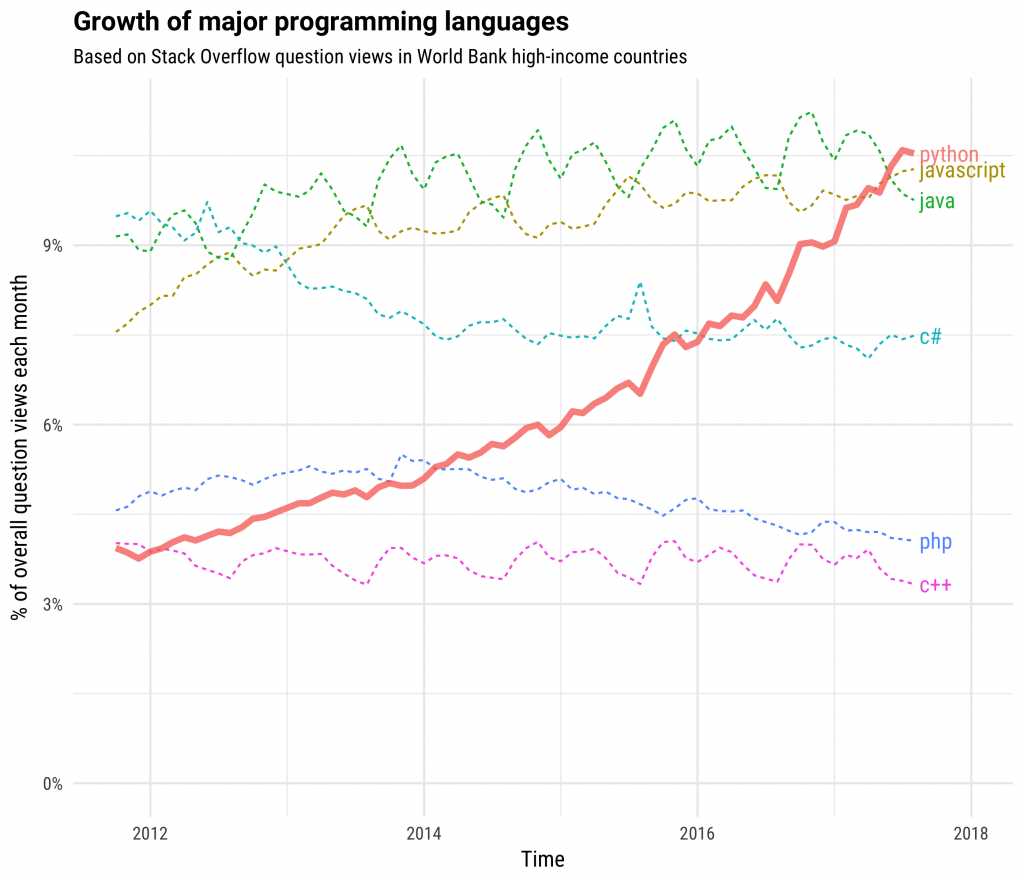
\includegraphics[scale=0.36]{images/languages-var.png}
    \caption{Évolution de la popularité des langages les plus utilisés entre 2012 et 2018}
    \label{fig:lang-var}
\end{figure}
\vspace{5pt}
Python a atteint une popularité semblable à Java ces dernières années, et semble conforter sa première place au classement de l'\textbf{IEEE}, devant Java.

Pour le langage, le bon choix technique semble être \textbf{Python}, les performances offertes par l'implémentation native de \textbf{SpaCy} étant bien meilleure que sur du Java, tout en ayant les avantages de Java. Le langage n'est évidemment pas le seul critère de distinction entre ces deux bibliothèques : la fréquence de mise à jour, l'ouverture aux autres langues ou encore l'outillage autour du produit sont à prendre en compte.
\label{section 3.1.1}

\subsubsection{Deux philosophies}
Les buts recherchés derrière la création des deux bibliothèques sont différents : Stanford Core NLP, dont la première version date de 2010, vise à montrer l'état de l'art dans le TLN. Elle rassemble beaucoup de fonctionnalités, essentiellement pour l'anglais, et atteint de meilleures niveaux de précision que les bibliothèques standards. Le but d'\textbf{Explosion AI} avec \textbf{SpaCy}, est d'offrir un outil industriel facilement utilisable pour tout les cas d'applications : ChatBot, corrections de formulaires, indexation de contenu, etc. Basé en partie sur les travaux mené par le groupe de recherche \textbf{Stanford NLP} et la première version datant de 2015, elle propose les fonctionnalités les plus génériques et sur lesquelles l'efficacité est prouvée. \textbf{Explosion AI}, qui développe SpaCy, s'attache également à intégrer le plus de langues possibles, contrairement à Core NLP qui se concentre sur l'anglais.
\newline

Voici un tableau récapitulatif des différents traitements proposés par les bibliothèques :
\vspace{10pt}
\begin{table}[H]
    \centering
    \begin{tabular}{| p{0.4\linewidth} | c | c | c |}
        \hline 
        \textbf{Fonctionnalités} &\textcolor{red}{Core NLP} &\textcolor{blue}{SpaCy} &\textcolor{orange}{NLTK}\\
        \hline
        \hline 
        \textit{Neural network models} &O &O &X\\
        \hline 
        \textit{Integrated word vectors} &X &O &X\\
        \hline 
        \textit{Multi-language support} &O &O &O\\
        \hline 
        \textit{Tokenization} &O &O &O\\
        \hline
        \textit{Part-of-speech tagging} &O &O &O\\		
        \hline 
        \textit{Sentence segmentation} &O &O &O\\
        \hline 
        \textit{Dependency parsing} &O &O &X\\
        \hline
        \textit{Lemmatization} &O &O &O\\
        \hline 
        \textit{Entity recognition} &O &O &O\\
        \hline 
        \textit{Entity linking} &O &X &X\\
        \hline 
        \textit{Coreference resolution} &O &X &X\\
        \hline 
        \textit{Open Information Extraction} &O &X &X\\
        \hline 
        \textit{Sentiment analysis} &O &X &X\\
        \hline
    \end{tabular}
    \caption{Tableau comparatifs des fonctionnalités proposées par les bibliothèques standards}
    \label{tab:nlp-compare}
\end{table}
\vspace{5pt}

Ce tableau est inspiré de celui proposé dans la \href{https://spacy.io/usage/facts-figures}{documentation de SpaCy}; il le complète et le corrige avec l'état acutelle des bibliothèques. NLTK, \textit{Natural Language Toolkit} est la bibliothèque historique de TLN en Python : la première version date de 2001. En tant que référence de longue date dans le domaine du TLN, il est placé dans le tableau à titre de comparaison avec les autres bibliothèques.
\newline

Du fait de son orientation recherche, Core NLP offre davantage de fonctionnalités en anglais, notamment \textit{Entity Linking} et \textit{Coreference resolution}, traitements utiles dans notre cas d'utilisation. Ces fonctionnalités que n'a pas SpaCy sont assez dépendantes du contexte d'utilisation~: \textit{Entity Linking} dépend de la base de données utilisée. \textit{Open Information Extraction}, qui s'attache à extraire des triplets sujet-relation-objet d'un texte dépend de l'ontologie utilisée. Ces fonctionnalités ne sont donc pas réutilisables dans des contextes spécifiques, l'objectif de la bibliothèque étant de montrer que ces traitements sont possibles, et non de fournir un outil. C'est l'objectif affiché par SpaCy, et c'est pourquoi elle intègre des dictionnaires de vecteurs de mots.
\newline

La différence entre les deux bibliothèques apparaît également dans la possibilité de personnaliser et d'adapter les fonctionnalités à nos besoins. D'une part, la documentation de SpaCy est plus fournie et plus facile d'utilisation que celle de Core NLP. Cette dernière ne détail pas toute les fonctionnalités de l'outil, mais fait davantage référence à des articles de recherche. Cela permet une meilleure compréhension des mécanismes utilisés dans le TLN, mais nécessite davantage de temps pour maîtriser l'utilisation de l'outil. Elle offre de plus davantage de personnalisation, avec notamment un outil générique, \href{https://stanfordnlp.github.io/CoreNLP/tokensregex.html}{\textit{TokensregexAnnotator}}, qui fournit un langage spécifique à la bibliothèques pour effectuer des traitements. L'outil équivalent de SpaCy, \href{https://spacy.io/usage/rule-based-matching}{\textit{Matcher}} n'est pas aussi générique, et l'efficacité est préférée~: le format utilisé est standard (\textbf{jsonl}) et la grammaire reste simple.
\newline

Pour notre cas d'étude, deux aspects sont à étudier plus précisément : la généralisation des traitements aux autres langues, l'organisme \textbf{Eurostat} étant intéresse par le projet, et les différences sur la reconnaissance d'entités nommées.
\label{section 3.1.2}

\subsubsection{L'ouverture du service}
Bien que la \autoref{tab:nlp-compare} montre un support multilingue des deux bibliothèques, elle est à détaillé. Le groupe de recherche de Stanford s'est en effet concentré sur la langue de Shakespeare, et offre des modèles pour l'Arabe, le Chinois, le Français, l'Allemand et l'Espagnol. Ces modèles n'offre de plus pas toutes les fonctionnalités, comme on peut le voir dans ce tableau issu de la \href{https://stanfordnlp.github.io/CoreNLP/human-languages.html}{documentation de Core NLP} :
\vspace{10pt}
\begin{table}[H]
    \centering
    \begin{tabular}{| p{0.35\linewidth} | c | c | c | c | c | c |}
        \hline
        \textbf{Traitements} &AR &ZH &EN &FR &DE &ES\\
        \hline 
        \hline
        \textit{Tokenization} &O &O &O &O &X &O\\
        \hline
        \textit{Part-of-speech tagging} &O &O &O &O &O &O\\		
        \hline 
        \textit{Sentence segmentation} &O &O &O &O &O &O\\
        \hline 
        \textit{Dependency parsing} &X &O &O &O &O &X\\
        \hline
        \textit{Lemmatization} &X &X &O &X &X &X\\
        \hline 
        \textit{Entity recognition} &X &O &O &X &O &O\\
        \hline 
        \textit{Entity linking} &X &O &O &X &X &X\\
        \hline 
        \textit{Coreference resolution} &X &O &O &X &X &X\\
        \hline 
        \textit{Open Information Extraction} &X &X &O &X &X &X\\
        \hline 
        \textit{Sentiment analysis} &X &X &O &X &X &X\\
        \hline
    \end{tabular}
    \caption{Tableau récapitulatif des traitements de Core NLP en fonction de la langue}
    \label{tab:corenlp-lang}
\end{table}
\vspace{10pt}

Pour le cas présent, on s'intéresse d'abord au français, puis à l'anglais et aux autres langues européennes. La bibliothèque offre pour ces dernières le traitement de REN, excepté pour le français. Les quatre traitements proposés ont toutefois un potentiel via l'utilisation des \textit{Tokensregex}.
\newline

 Bien que le projet soit OpenSource et disponible sur \href{https://github.com/stanfordnlp/CoreNLP}{Github}, les contributions extérieures sont moins nombreuses que sur \href{https://github.com/explosion/spaCy}{SpaCy}. Explosion AI encourage vivement les contributions extérieures, notamment en ce qui concerne le support d'autres langues. La bibliothèque propose à ce jour les fonctionnalités principales pour un large panel de modèles, avec parfois plusieurs modèles par langues :
 \vspace{10pt}
\begin{figure}[H]
    \centering
    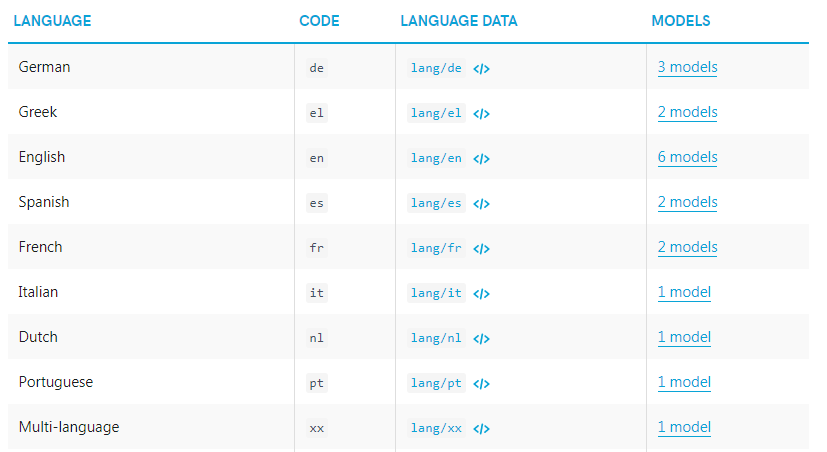
\includegraphics[scale=0.7]{images/spacy-lang.png}
    \caption{Tableau récapitulatif des modèles disponibles pour SpaCy, tiré de la \href{https://spacy.io/usage/models}{documentation}}
    \label{fig:spacy-lang}
\end{figure}
\vspace{10pt}

Les langues listées ci-dessus proposent toutes les traitements de SpaCy listés \autoref{tab:nlp-compare}. Pour le modèle multi-lingues (ML), il propose uniquement la REN pour l'anglais, l'allemand, l'espagnol, le français, l'italien, le portugais et le russe. D'autres modèles sont à l'étude et utilisables : ils couvrent plus d'un vingtaines de langues d'Asie et d'Europe. Les ajouts de supports de langues et autres mises à jours sont assez fréquents sur SpaCy. La communauté autour de l'outil est très active et de nombreuses petites améliorations apparaissent petit à petit. Comme on peut le voir sur le \href{https://github.com/explosion/spaCy}{Github} du projet, toutes les améliorations, idées d'améliorations et bugs sont publiés. J'ai notamment eu l'occasion de proposer une idée d'amélioration pour le format de sortie des données. Les mainteniciens de la bibliothèques semblent très réactifs et à l'écoute de la communauté, ce qui facilite à la fois la visibilité de la bibliothèque et son ouverture aux autres langues. A titre d'exemple, Explosion AI sort actuellement une mise à jour tout les un à deux mois. À titre de comparaison, la dernière mise à jour de Stanford Core NLP date d'octobre 2018.
\newline

N'ayant pas une grande expertise sur le TLN et sur les autres langues en général, le bon choix, afin de profiter d'une communauté active et de nouvelles fonctionnalités fiables, semble être SpaCy. Il reste cependant à aborder l'aspect central du projet~: la construction d'un pipeline de reconnaissance d'entités nommées.
\label{section 3.1.3}

\subsubsection{La REN dans les deux bibliothèques}
Bien que le sujet soit déjà abordé partie \ref{section 2.2.4} avec Core NLP, certains points concernant la REN, notamment avec SpaCy restent à aborder. 
\newline

SpaCy offre les mêmes fonctionnalités pour reconnaître ses propres entités nommées, à savoir la reconnaissance à base de règles et celle à base de réseaux de neurones. Pour les règles, SpaCy intègre un composant, \textit{EntityRuler}, qui permet de faire directement de la REN avec les règles, la où Core NLP est plus général avec les \textit{Tokensregex}. La syntaxe est plus simple avec SpaCy, qui utilise un format standard (des exemples sont donnés en annexe).
\newline

La bibliothèque propose également deux modèles de REN, qui reconnaissent les entités de type personne, lieux, organisation et divers. Quelques rapides tests montrent que le modèle \textit{small} a ses limites, notamment sur le \textit{POS-tagging}, tandis que le modèle \textit{medium} reconnaît assez généralement les trois premiers types d'entités. Quasiment aucun concept statistiques n'est reconnu en tant qu'entité diverse par le modèle. Un test a également été réalisé à partir d'un modèle de REN compatible avec Core NLP et entraîné par \href{http://lab.kbresearch.nl/static/html/eunews.html}{Europeana}. TODO : compléter
\newline

Là encore, SpaCy semble plus adapté pour construire un service de reconnaissance d'entités nommées, sa simplicité d'utilisation et son efficacité étant nettement meilleure que ce qui est proposé par Core NLP. C'est donc assez naturellement que \textbf{SpaCy} a été choisi pour construire le service. 
\label{section 3.1.4}

\subsection{L'architecture du projet}

\subsubsection{Une architecture micro-service}
Pour faciliter l'intégration avec d'autres services qui pourrait être développés ultérieurement (voir section \ref{section 2.1.4}), j'ai fait le choix de construire un web-service sous forme d'\textbf{API REST} qui effectue la REN. Il s'impose assez naturellement : d'une part parce que c'est un standard du web, et d'autre part parce qu'il s'adapte parfaitement bien au cas d'usage.
\newline

L'objectif à court terme est de construire un service applicatif et un service utilisateur. Les deux services s'articulent comme suit :
\vspace{20pt}
\begin{figure}[H]
    \centering
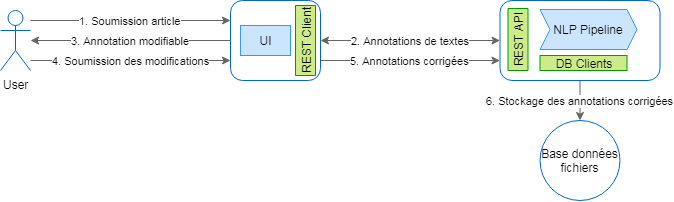
\includegraphics[scale=0.62]{images/Archi-pipeline-web.png}
    \caption{Articulation des Web-services à mettre en place}
    \label{fig:archi-pipeline-web}
\end{figure}

Ce choix d'architecture à été guidé par une réflexion sur les fonctionnalités assurées par le service. Ce dernier doit se concentrer principalement sur la REN, et non sur le format des données d'entrée/sortie. C'est pourquoi le format des données échangées doit rester simple et standard : le choix s'est porté sur du \textbf{json}, \textit{JavaScript Object Notation}. Python propose en effet nativement des objets similaires ainsi que des bibliothèques associées très faciles d'utilisation. Bien qu'il soit incomplet, un résultat des traitements au format json est donnée par une fonction de la bibliothèque SpaCy. J'ai d'ailleurs soumis une \textit{issue} sur le \href{https://github.com/explosion/spaCy/issues/3987}{Github} du projet SpaCy, qui propose d'améliorer ce rendu. Je n'ai à l'heure actuelle pas trouvé le temps de l'implémenter, cela nécessitant une connaissance approfondie de l'implémentation de la bibliothèque et de \textbf{Cython}.

Dans le cas d'une utilisation avec les publications de l'Insee, l'idée est de laisser la gestion du format des publications au service utilisateur, qui fait alors plusieurs appels au serveur applicatif pour annoter la totalité d'une publication. Cela permet de ne pas perdre les informations liées au format. Ce choix a de plus l'avantage de laisser le serveur applicatif sans état, \textit{stateless}, ce qui facilite la gestion de plusieurs instances et donc le passage à l'échelle. Cela est une qualité importante du Web-service~: les utilisations possibles, comme décrites section \ref{section 2.1.3} sont nombreuses et il est nécessaire de maintenir une bonne disponibilité. Cela est d'autant plus important que les traitements prennent du temps, environ quelques centaines de millisecondes~: le nombre d'instances à déployer peut donc vite augmenter. 
\newline
\label{section 3.2.1}

\subsubsection*{Architecture des services}
L'architecture du service d'application ressemble au premier service décrit section \ref{section 2.2.5}. Elle intègre cependant quelques changements, notamment sur l'ajout des entités à reconnaître :
\vspace{10pt}
\begin{figure}[H]
    \centering
    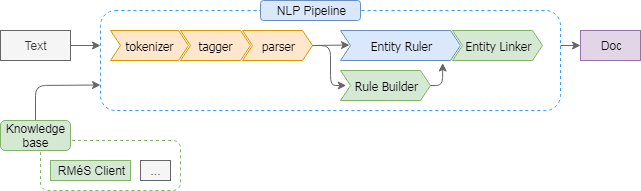
\includegraphics[scale=0.7]{images/InspaCy-archi.png}
    \caption{Architecture du service de REN}
    \label{fig:inspacy-archi}
\end{figure}
\vspace{10pt}

Comme pour la \autoref{fig:premier-pipeline}, les éléments de couleur bleus sont ceux fournis par SpaCy que je personnalise, les éléments en verts sont ceux crées par moi-même et les éléments de couleur orange sont ceux que je ré-utilise sans les modifier. Dans le premier pipeline, l'ajout de nouvelles entités à reconnaître se faisait «~à la main~», c'est-à-dire en ajoutant une ligne au fichier des entités nommées. Dans l'architecture décrite ci-dessus, l'idée est de proposer une base de connaissance sous forme de clients de base de données. Ces clients récupèrent au lancement du programme les libellés et identifiants des entités nommées de leur base pour les traiter via un pipeline TLN et créer des règles. Quatre composants permettent de créer ces règles : \textit{Tokenizer}, \textit{Tagger} et \textit{Parser}, dont les instances sont partagées avec le pipeline principal au lancement du serveur, et le composant \textit{Rule Builder}. Ce dernier composant récupère l'annotation issue du pipeline pour créer les règles et les injecter directement dans le composant \textit{Entity Ruler}. Cela évite de stocker les règles sur le disque, comme cela est le cas avec le premier service.
Le second changement se situe au niveau du composant \textit{Entity Linker}. Bien qu'une \textit{issue} sur le dépôt \href{https://github.com/explosion/spaCy/issues}{Github} semble indiqué que le composant est en cours d'implémentation, j'ai préféré en créer un moi-même afin de pouvoir avancer dans l'implémentation. Les traitements de reconnaissance et de ceux de liens avec des base de données sont séparés dans ce pipeline, afin de pouvoir tester différentes bases de connaissances. Le cas des concepts géographiques en est un bon exemple.
\newline

La méthode de REN ne change pas dans ce service : j'intègre toutefois la possibilité de générer des règles plus simples que celle décrite section \ref{section 2.2.5}. Ces types de règle supplémentaires cherchent les libellés exacts, en prenant ou non en compte la casse. Cela a pour but de pouvoir ajouter facilement des entités plus spécifiques, comme des organisations (Ministères, Eurostat) ou encore des lieux. Bien que SpaCy propose des modèles de REN pour le français capable de reconnaître ces concepts, je fais le choix de ne pas les utiliser~: les composants \textit{Entity Ruler} et \textit{Entity Recognizer} fonctionnent mal ensemble (voir section \ref{section 3.1.4}). Cela implique nécessairement d'intégrer différents types de règles pour reconnaître d'autres types d'entités (nombres, noms propres). 
\newline

L'interface utilisateur doit permettre à un rédacteur d'obtenir un retour sur sa publication, et d'éditer les annotations du service de REN. Il devra donc avoir un module à part pour gérer le format des publications. Voilà les fonctionnalités attendues :
\begin{itemize}
    \item L'interface doit permettre d'entrer du texte directement sur la page, ou de soumettre un fichier depuis le disque local. On doit pouvoir spécifier le format du fichier et sa grammaire associée. Pour le moment, un module pour le XML suffit.
    \item À partir de la réponse du serveur REN, l'interface doit présenter le texte comme un ensemble de boutons, chaque bouton correspondant à un token. Ces boutons doivent être de couleurs différentes si ce sont des entités nommées (voir \href{https://spacy.io/usage/visualizers#ent}{displaCy}).
    \item L'utilisateur doit pouvoir rassembler/désassembler les tokens pour les annoter en tant qu'entités nommées, ainsi que choisir le type d'entités nommées (Concept statistique, Organisation, Lieux, Dates).
    \newline
\end{itemize}

L'architecture des services webs établie, il a fallut choisir les frameworks qui facilitaient l'implémentation des deux services.

\label{section 3.2.1 - Architecture des services}

\subsubsection{Les technologies utilisées}
Le choix s'est très vite fixé pour l'implémentation du service de REN sur \href{https://github.com/pallets/flask}{Flask}. La facilité d'utilisation, la rapidité avec laquelle on peut mettre en place un service, tout en garantissant le passage en production, le framework est tout indiqué. Ayant peu de connaissances sur le développement web \textit{front-end}, il était difficile pour moi d'effectuer un choix de technologies pour l'interface. \textbf{Angular}, \textbf{React}, \textbf{Vue.js}, de nombreux frameworks javascripts existent, et il n'est donc pas évident de se fixer sur un outil. J'ai a cet occasion été conseillé par Eric de la DIIT (voir section \ref{section 1.1.2}) et Renaud Genevois de la cellule architecture, principal développeur d'\textit{Onyxia-IHM}. Cette dernière a été développée en React et j'ai pu explorer son code source.
\label{section 3.2.2}

\subsubsection*{Flask \& Python : créer un web service en une heure}
La principale qualité de Flask et des frameworks Python en général est la rapidité avec laquelle on peut créer et déployer un web-service. Afin d'en faire un web-service, il a suffit d'ajouter un simple fichier Python décrivant les routes et méthodes HTTP associées. Comparativement à \textbf{JAX-RS}, framework standard Java pour mettre en place une API REST, ou encore à \textbf{Javalin}, plus récent, l'implémentation avec Flask est beaucoup plus légère. La où les framework Java propose des interfaces à implémenter, des annotations et des dépendances à choisir, Flask requiert une simple ligne de code et des décorateurs (équivalent des annotations Java).
\newline

Flask intègre également un outil de \textit{templating html}, \textbf{Jinja2}, qui permet de créer une petite interface web. J'ai donc pu intégrer rapidement une interface pour tester à la main le service. J'y ai ajouté pour le moment des options pour pouvoir aisément vérifier les résultats du pipeline. Ce framework se complète très bien avec \textbf{SpaCy}~: la bibliothèque TLN intègre depuis peu un outil fournissant un visuel HTML pour les résultats de REN et de dépendances. Cela permet avec Jinja2 une intégration du rendu généré par le module \textbf{displacy} directement dans la page HTML. C'est la encore une illustration de la rapidité avec laquelle on peut mettre en place un web-service avec \textbf{SpaCy} et \textbf{Flask}. Voilà un aperçu de la page de démonstration réalisée avec ces deux outils~:
\begin{figure}[H]
    \centering
    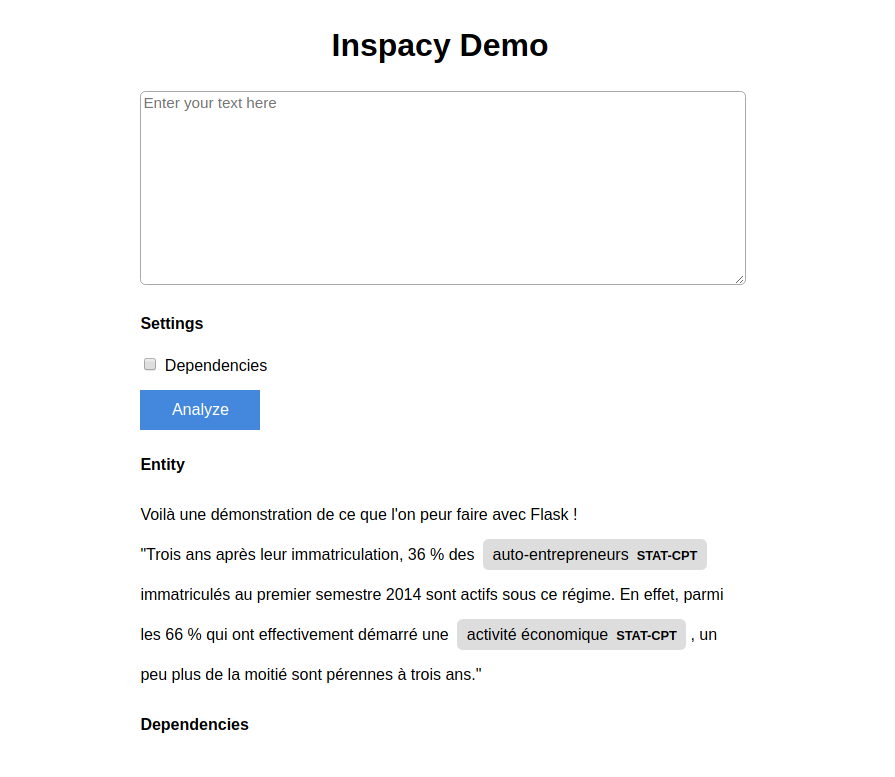
\includegraphics[scale=0.6]{images/inspaCy-demo.png}
    \caption{Capture du service de reconnaissance d'entités nommées développé avec Flask}
    \label{fig:demo-inspaCy}
\end{figure}

J'ai pu grâce à Flask, mettre en place le web service en une journée : création des routes, formatage des données et interface minimaliste. Cela rejoint l'analyse des différences relevées entre Python et Java section \ref{section 3.1.1}~: Python est très efficace pour prototyper et tester, sans avoir à se soucier d'aspects bas niveau, comme la gestion de la mémoire, les entrés-sorties ou encore la gestion des dépendances.
\label{section 3.2.2 - Flask}

\subsubsection*{React}
Le choix pour l'interface utilisateur s'est finalement portée sur React. Framework javascript le plus populaire acutellement, comme le montre cet article de \href{https://stackoverflow.blog/2018/01/11/brutal-lifecycle-javascript-frameworks/}{stackoverflow}, il permet de créer une interface utilisateur sous forme de composants. Utilisant un DOM virtuel, \textit{Document Object Model}, il permet d'intégrer des composants complexes dans une interface, et ce de façon dynamique. Développer une interface consiste donc simplement à placer des composants et à créer les fonctions définissant les comportements spécifiques au cas d'usage. De nombreuses bibliothèques de composants React existent à ce jour (\textbf{Material-UI}, \textbf{React-bootstrap}, \textbf{React toolbox}, etc.), offrant toutes sortes de boutons, menus et éléments d'interactions. N'ayant jamais développé de projet en Javascript, cela m'a permis en très peu de temps de faire une petite interface pour un projet associatif.
\newline

J'ai cependant manqué de temps pour obtenir une interface fonctionnelle, que ce soit pour mon projet associatif ou pour l'interface utilisateur. Bien que Javascript soit assez accessible pour quelqu'un ayant développer dans d'autres langages, le framework React nécessite une connaissance approfondie du développement \textit{Front-end}~: gestion du cache, appels asynchrones à une API ou encore découpage de l'application en composants, il me reste encore beaucoup de choses à apprendre sur \textbf{React} pour être efficace sur le développement d'une interface utilisateur. Ne disposant pas du temps suffisant pour développer l'interface, et dans la mesure où l'Insee dispose d'agents maîtrisant le framework, je me suis donc contenter de laisser les spécifications.
\newline

Motivé et éclairé par le pipeline mis en place pour le premier service de REN, j'ai pu pour ce second programme apprécier les outils de la plateforme Innovation qui m'ont permis de développer en continu.
\label{section 3.2.2 - React}

\subsubsection{Intégration dans la démarche DevOps}
Tests, mise en service et déploiement de l'application : j'ai voulu cette fois-ci automatiser tout le processus de vie du web-service, jusqu'à un déploiement sur la plateforme innovation. Je me suis cependant très vite heurté à un problème majeur~: la bibliothèque \textbf{SpaCy} n'est pas compatible avec le poste sur lequel je travaille. Manquant de temps, je me suis rapidement adapté en travaillant sur mon ordinateur personnel. N'étant pas relié au réseaux, il est difficile d'accéder au \textbf{GitLab} et de manière général à la plateforme Innovation. J'ai donc travaillé sur \textbf{Github}, et effectuer un lien manuel avec GitLab à partir de mon poste de travail. \textbf{Git} étant un mécanisme de versionnement non centralisé, il permet d'avoir plusieurs dépôts distants~: dans le cas du dépôt de mon poste de travail, un dépôt Github et un dépôt GitLab. Dans l'idéal, il aurait fallut intégrer un \textit{web hook} sur Github, afin que chaque mise à jour du dépôt lance le pipeline CI/CD sur le dépôt GitLab. \textbf{Github Action} fournit un outil spécifique pour lancer des jobs sur un GitLab depuis un dépôt Github.
\newline

Bien que je n'ai pas eu le temps de mettre en place le processus d'intégration et de déploiement en continu, j'ai préparé le terrain~: afin d'effectuer le deploiement sur la plateforme innovation, il est nécessaire d'ajouter au projet plusieurs fichiers~:
\vspace{5pt}
\begin{itemize}
    \item Une image Docker~: c'est l'environnement d'exécution de l'application. Pour l'immense majorité des services, cet environnement est basé sur une distribution linux légère, auquel on ajoute les bibliothèques et outils dont a besoin l'application pour s'exécuter correctement. Dans le cas du service de REN, on a donc besoin d'un environnement contenant \textbf{Python 3.6} ou toute version ultérieure, ainsi que les bibliothèques \textbf{Python} utilisées dans le projet (SpaCy, Flask, Flask-CORS, requests). Le choix est fait d'intégrer ces bibliothèques directement dans l'image, plutôt que de les télécharger à chaque lancement du conteneur~: cela augmente le volume de l'image Docker mais permet de gagner en rapidité de lancement du conteneur. SpaCy est en effet assez lourd et nécessite de plus les modèles de TLN, qui sont eux aussi volumineux. J'ai donc pris le temps de construire cette image Docker, afin de faciliter l'avancement futur du projet.
    \vspace{5pt}
    \item Un contrat de déploiement~: il spécifie comment le conteneur doit être déployé sur la plateforme. Ressources à allouer, ports à exposer, réseau Docker sur lequel le déployer ou encore variables d'environnements à ajouter~: toutes ces informations sont données à \textbf{Marathon} qui déploie le service sur un nœud du cluster. 
    \vspace{5pt}
    \item Le fichier décrivant le pipeline~: \textit{.gitlab-ci.yml} pour GitLab, il spécifie les étapes du pipeline, les environnements à utiliser et les commandes shells à exécuter.
    \newline
\end{itemize}

J'ai donc préparer au mieux la mise en place d'un pipeline de déploiement continu, afin de faciliter l'intégration de d'autres fonctionnalités, telles que l'ajout d'entités nommées ou l'ajout d'un client \textbf{Minio} pour stocker les données d'entraînement. Une évaluation des données d'entraînement est également à l'étude, afin de savoir si l'on peut lancer un entraînement.
\label{section 3.2.3}

\subsubsection*{Conclusion}
Le développement de ce service, de la méthode à la mise en service, m'a beaucoup apporté sur la mise en production d'applications. Tant sur les choix d'outils que sur les choix d'architecture, j'ai eu l'occasion de mobiliser les compétences acquises dans ma formations, et plus particulièrement dans mon projet de fin d'étude.

\newpage
\section{Bilan \& perspectives}
Ce projet a finalement abouti à l'élaboration de deux services de reconnaissance d'entités nommées~: un premier prototype fonctionnel, et un second service, plus industriel. Ils montrent tout deux des résultats encourageants, et qui servira tant aux rédacteurs des publications qu'à l'équipe en charge du référentiel des métadonnés statistiques. Cela m'a de plus permis de préciser mon projet professionnel, en explorant à la fois les thématiques de traitements de langages naturels, de développement web et la thématique DevOps.

\subsection{Le livrables et les résultats actuels}
Les livrables du projet, disponibles sur \href{https://github.com/Mardelor?tab=repositories}{Github}, sont au nombre de trois~: les deux services de REN et ce présent rapport.
\newline

Le premier service permet à ce jour de repérer les concepts de la base RMéS, et de générer un rendu XML et un rendu HTML d'une même publication. Un pipeline GitLab permet déjà de tester automatiquement le programme sur n'importe quelle publication figurant dans la base de données au format XML. Il donne une bonne vision de ce que l'on peut faire en TLN sur les publications de l'Insee, même s'il a quelques lacunes.
\newline

Une analyse du programme sur environ 650 publications, dont chacune fait trois à quatre pages a été menée. Il s'agit de rechercher quels concepts sont repérés dans le corpus, sous quelles formes et à quelle fréquence. On constate que la moitié des concepts est repérée sur les 1162 qui sont présents dans la base RMéS. Pour une majorité d'entre eux, ils ne sont trouvés moins de dix fois dans le corpus. Pour les concepts généraux en revanche, comme «~salaire~», «~commerce~» ou «~productivité~», on retrouve plusieurs formes et avec un nombre d'occurrences allant de quelques dizaines à quelques centaines.

Il est difficile de déterminer si les concepts qui n'apparaissent pas ne sont tout simplement pas mentionnés ou si cela est dû aux lacunes du pipeline. Ce que l'on peut en conclure en revanche, c'est que les concepts généraux sont cités avec des formes diverses. Cela pointe le fait que certains concepts mériteraient peut-être d'avoir des sous-concepts, plus spécifiques.
\newline

Le second service est plus aboutit~: construit pour pouvoir être utilisé sur le Web, il ne permet cependant pas, à l'heure actuelle, d'effectuer les tests sur les publications. Il dispose en revanche d'une interface pour soumettre du texte au pipeline, et ainsi rapidement vérifier si un concept est reconnus dans un certain contexte. Cette interface inclus également l'affichage des dépendances, permettant de résoudre les dysfonctionnements plus rapidement. Il est également adressable en HTTP et peut fournir le résultat du pipeline en JSON. Je n'ai malheuresement pas eu le temps de mettre en place un pipeline GitLab. J'ai cependant créer une image Docker sur laquelle l'application peut s'exécuter.
\newline

Bien que je n'ai pas pu finaliser la seconde application, j'ai pris soin de laisser une documentation, afin d'autres puissent faire aboutir le second service. 

\subsection{Perspectives d'amélioration}

Faire un client Java XSLT pour tester le pipeline SpaCy et ainsi comparer les résultats + réaliser l'interface utilisateur pour améliorer base RMéS \& se constituer une base d'apprentissage + finition de l'intégration sur la plateforme Innovation + amélioration du pipeline Java via le pipeline SpaCy + Exploration d'une méthode à base de \textit{Dependencies}.

\subsection{Apport dans mon projet professionnel}
\subsubsection{La vision apportée vis-à-vis de mon projet professionnel}
Travailler dans une grande entreprise, avec de l'agilité + difficulté de gérer la mission qui m'a été confiée tout en étant dans une équipe et en participant à leurs activités.

Travailler avec la DIIT et Franck Cotton pendant ces six mois a été très enrichissant pour moi. Cela m'a fait réfléchir sur le contexte dans lequel je veux travailler, ma relation avec les autres, et les sujets sur lesquelles j'aimerai travailler.
\newline

Le stage m'a tout d'abord apporté une confiance en moi. Être accueillit dans une structure de plus de 6000 agents a d'abord été intimidant. 
TODO : compléter avec équipe DIIT agile = stimulant + thématiques récentes + assez libre
Mais difficulté de faire partie de cette équipe tout en poursuivant ma propre mission. Difficultés à ce placer : aller voir les bonnes personnes, mais on m'a aidé et maintenant confiance ! poceblo
\newline

Vis-à-vis de ce que je veux faire, occasion de discuter avec pas mal de monde + mettre en pratique un certain nombre de compétences.

\subsubsection{Les compétences apportées}
DevOps ! Docker, Gitlab-CI, Framework de dev (Flask, Javalin, React,...) -> A la fois Ops et Data

Conclure sur le fait qu'aujourd'hui thèse CIFRE m'intéresse, car travailler sur des sujets récents en équipe est vraiment stimulant, ou équipe R\&D.

\subsubsection*{Conclusion}

\newpage

%--- conclusion ---%
\section*{Conclusion}
Par la description de mon environnement de travail, nous avons pu en premier lieu préciser les objectifs du stage. Nous avons ensuite exposé les résultats d'une étude sur la reconnaissance d'entités nommées qui a abouti à l'élaboration d'un premier prototype. Une comparaison des différents outils du traitement du langage naturel et du développement d'applications web a par la suite donné naissance à un second service. Cela a permis de présenter les résultats, apports et perspectives du projet, pour l'Insee comme pour moi.
\newline

Le service de développement de l'Insee à Montrouge m'a finalement fait une offre pour devenir développeur au sein de leurs équipes. Étant davantage attiré par le domaine de la recherche, j'ai préféré la décliner.
\newline

Le projet apporte des premiers résultats et une multitude d'applications possibles. Le Ministère de la Justice est par exemple intéressé par la reconnaissance d'entités nommées, afin d'anonymiser certains rapports.
\newpage

%----------------------------------------------------------------------------------%
%--- liste des figures et tableaux ---%
\listoffigures
\vspace{20pt}
\listoftables
\newpage

%--- bibliographie ---%
\bibliographystyle{unsrt}
\bibliography{biblio}
\newpage

%--- annexes ---%
\section*{Annexes}


\end{document}
